\documentclass{beamer}
\usepackage{amsmath}
\usepackage{amsthm}
\usepackage{amssymb}
\usepackage{cite}
\usepackage{xcolor}
\usepackage{enumitem}
\usepackage{graphicx}
\usepackage{caption}
\usepackage{mathtools}
\usepackage[makeroom]{cancel}
\usepackage{sansmathaccent}
\pdfmapfile{+sansmathaccent.map}


\title{Spatial Networks}
\subtitle{Generalized Network Models and Quantifying Spatial Embedding Strength}

\begin{document}
	\frame {
		\titlepage
	}
	\frame {
		\frametitle{Introduction}
		What is a network model?
		
		What are the uses of network models?
		
		When to consider (or not) spatial generalizations?
		
		\begin{figure}
		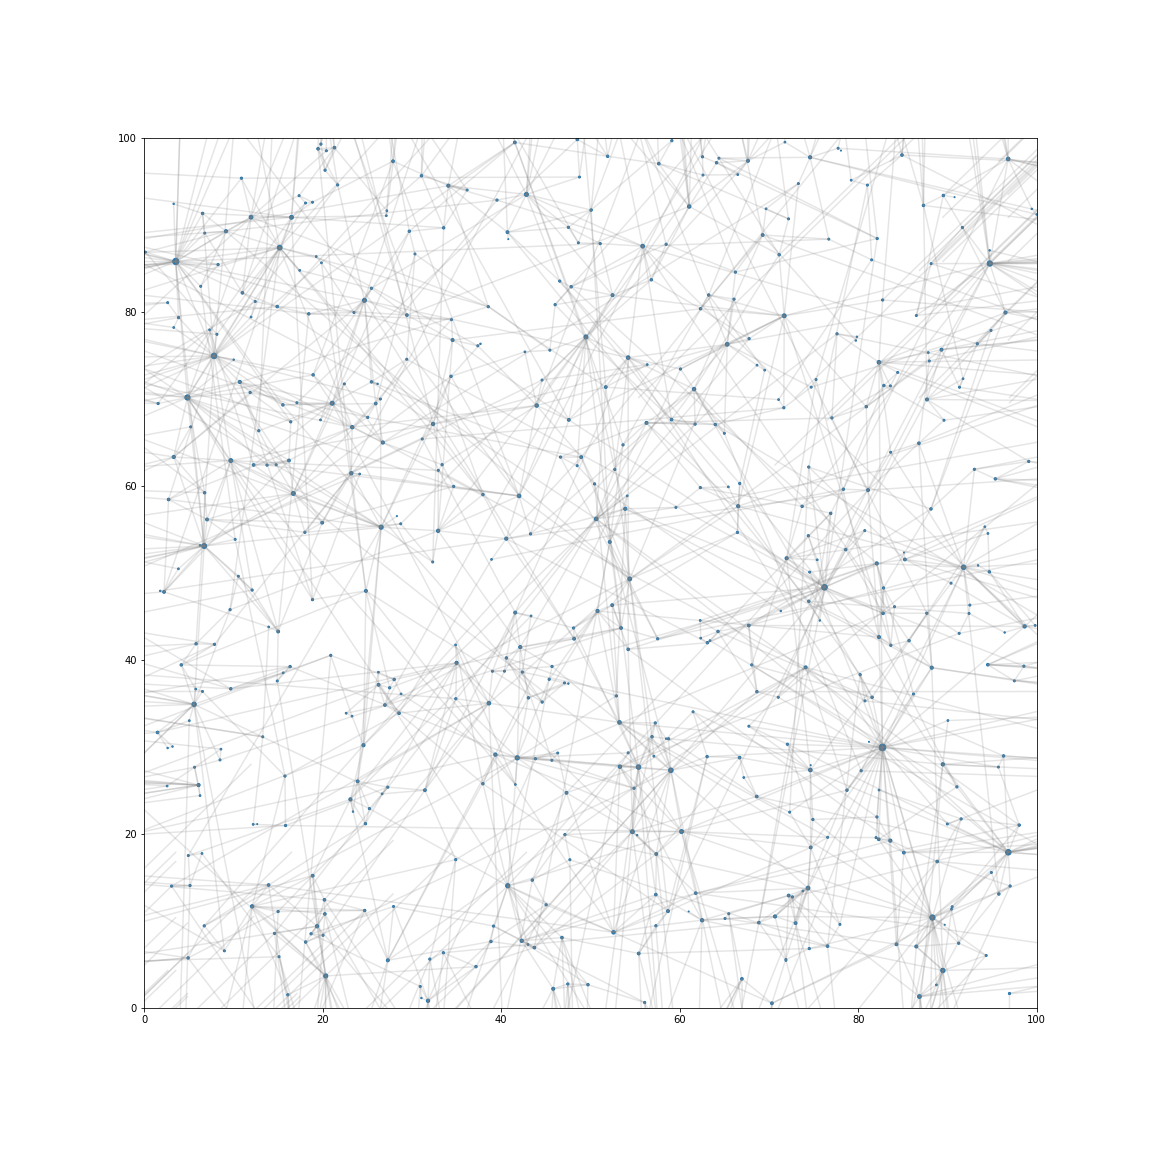
\includegraphics[width=0.7\linewidth]{../figures/configuration_network_example_beta_25.png}		
		\end{figure}
		%Network models can be thought of as a procedure to generate a network, and are designed to have certain features. For example, generating certain degree distribution, or mean clustering coefficient, or preserving some network features
		%Network models useful as
		% * way to generate network data to play with (e.g. run simulations, test dynamics and models)
		% * often in network science to see if some feature is significant, we use statistical analysis and ask if the feature appears often enough in comparison to some NULL MODEL
		% 	* ex. community detection
		%So makes sense to want to have good models to work with
		%Clearly, if you're using network models, you want to have networks that make sense to the situation you find yourself in
	}
	\frame{
		\frametitle{``Simple'' Spatial Generalization}
		\framesubtitle{How do we turn a non-spatial model into a spatial one?}
		Inclusion of a deterrence function:
		$$
		h(r_{i, j}) = r_{i, j}^{-\beta}, \beta > 0
		$$
		$r_{i, j}$ is the distance between nodes $v_i$ and $v_j$ \\		
		Use deterrence function to decrease likelihood of nodes that are far away to be adjacentskyp
		
		%Having a nice generalizable method of turning a non-spatial network into a spatial one is potentially a useful thing to have, since a lot of the reason people avoid spatial models is the added complexity
		%Generally, deterrence function is considered a decreasing function of distance
		%How we implement this deterrence function is unfortunately a choice we have to make
	}
	
	
	\frame{
		\frametitle{Network Models}
		\framesubtitle{Barabási-Albert (preferential attachment (PA)) model}
		Power-law degree distribution, ``rich get richer'' scheme	
		
		\textbf{Model description:}
		\begin{itemize}
			\item $\bullet$ Start with a ``seed'' network (e.g. 10-clique)
			\item $\bullet$ Evolve the network: at each time step add a new node. New node creates $m$ edges to nodes with probability proportional to the degree $k_j$ of existing node $k_j$
			\item $\bullet$ Continue until $T$ nodes added
		\end{itemize}
		
		
		Probability of forming edge from node $v_t$ at time $t$ to existing node $v_j$:
		$$
		p(v_t, v_j) = \frac{k_j}{\sum_{i}k_i}
		$$
	}
	\frame{
	    \frametitle{Network Models}
	    \framesubtitle{Spatial preferential attachment (SPA) model}
	    \textbf{Differences:}
	    \begin{itemize}
	    	\item $\bullet$ Network is embedded in $[0,1] \times [0,1]$ 2-dimensional space. Every new node is assigned a position uniformly at random
	    	\item $\bullet$ Edges are created proportional to degree $k_j$ of existing node and distance $r_{t,j}$.
	    \end{itemize}
	    
	    New probability:
	    $$
		p(v_t,v_j) = \frac{k_j}{\sum_i k_i}h(r_{t,j})\,.
		$$
	}
	\frame{
		\frametitle{Network Characteristics}
		
		\begin{itemize}
			\item $\bullet$ Mean local clustering coefficient: $c_i = \frac{2T(v_i)}{k_i(k_i - 1)}$
			\item $\bullet$ Mean geodesic distance: $L = \frac{\sum_{i \neq j}d(v_i, v_j)}{n(n-1)}$
			\item $\bullet$ Mean edge length
			\item $\bullet$ Degree assortativity: $r = \frac{\sum_{i,j}(A_{i,j}-k_i k_j/2m)k_i k_j}{\sum_{i,j}(k_i \delta_{i,j}-k_i k_j/2m)k_i k_j}$
		\end{itemize}
	}
	\frame {
		\frametitle{Network Models}
		\framesubtitle{SPA Characteristics}
		%\begin{figure}
		%	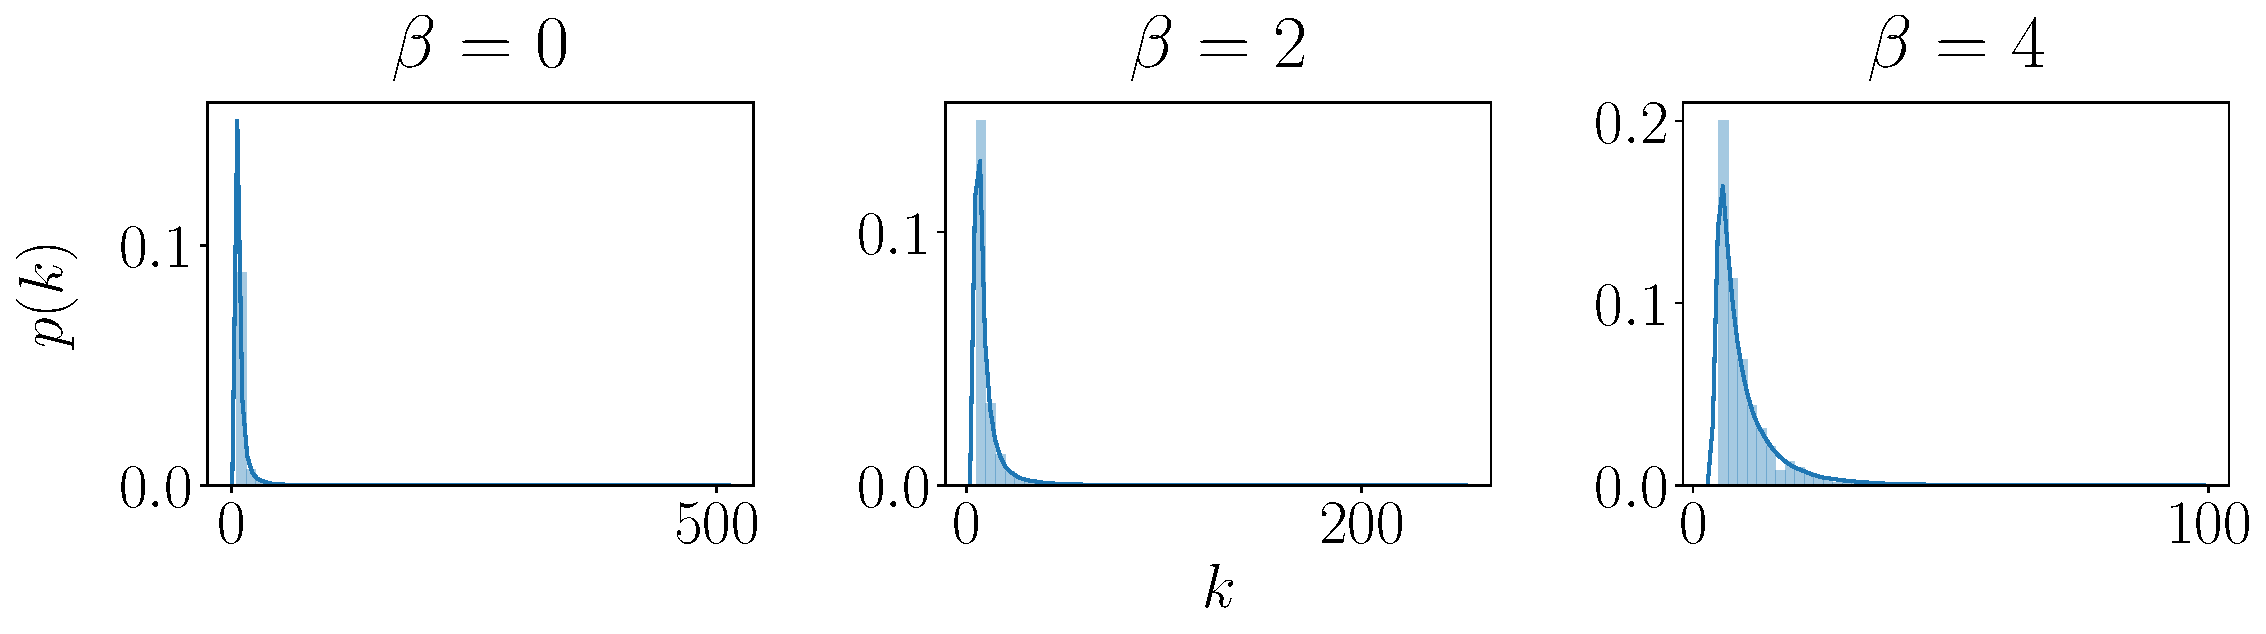
\includegraphics[width=0.5\linewidth]{../figures/preferential_attachment_degree_distribution.pdf}
		%	\caption{Degree distributions for $T=10000$}
		%\end{figure}
		
		\begin{figure}
			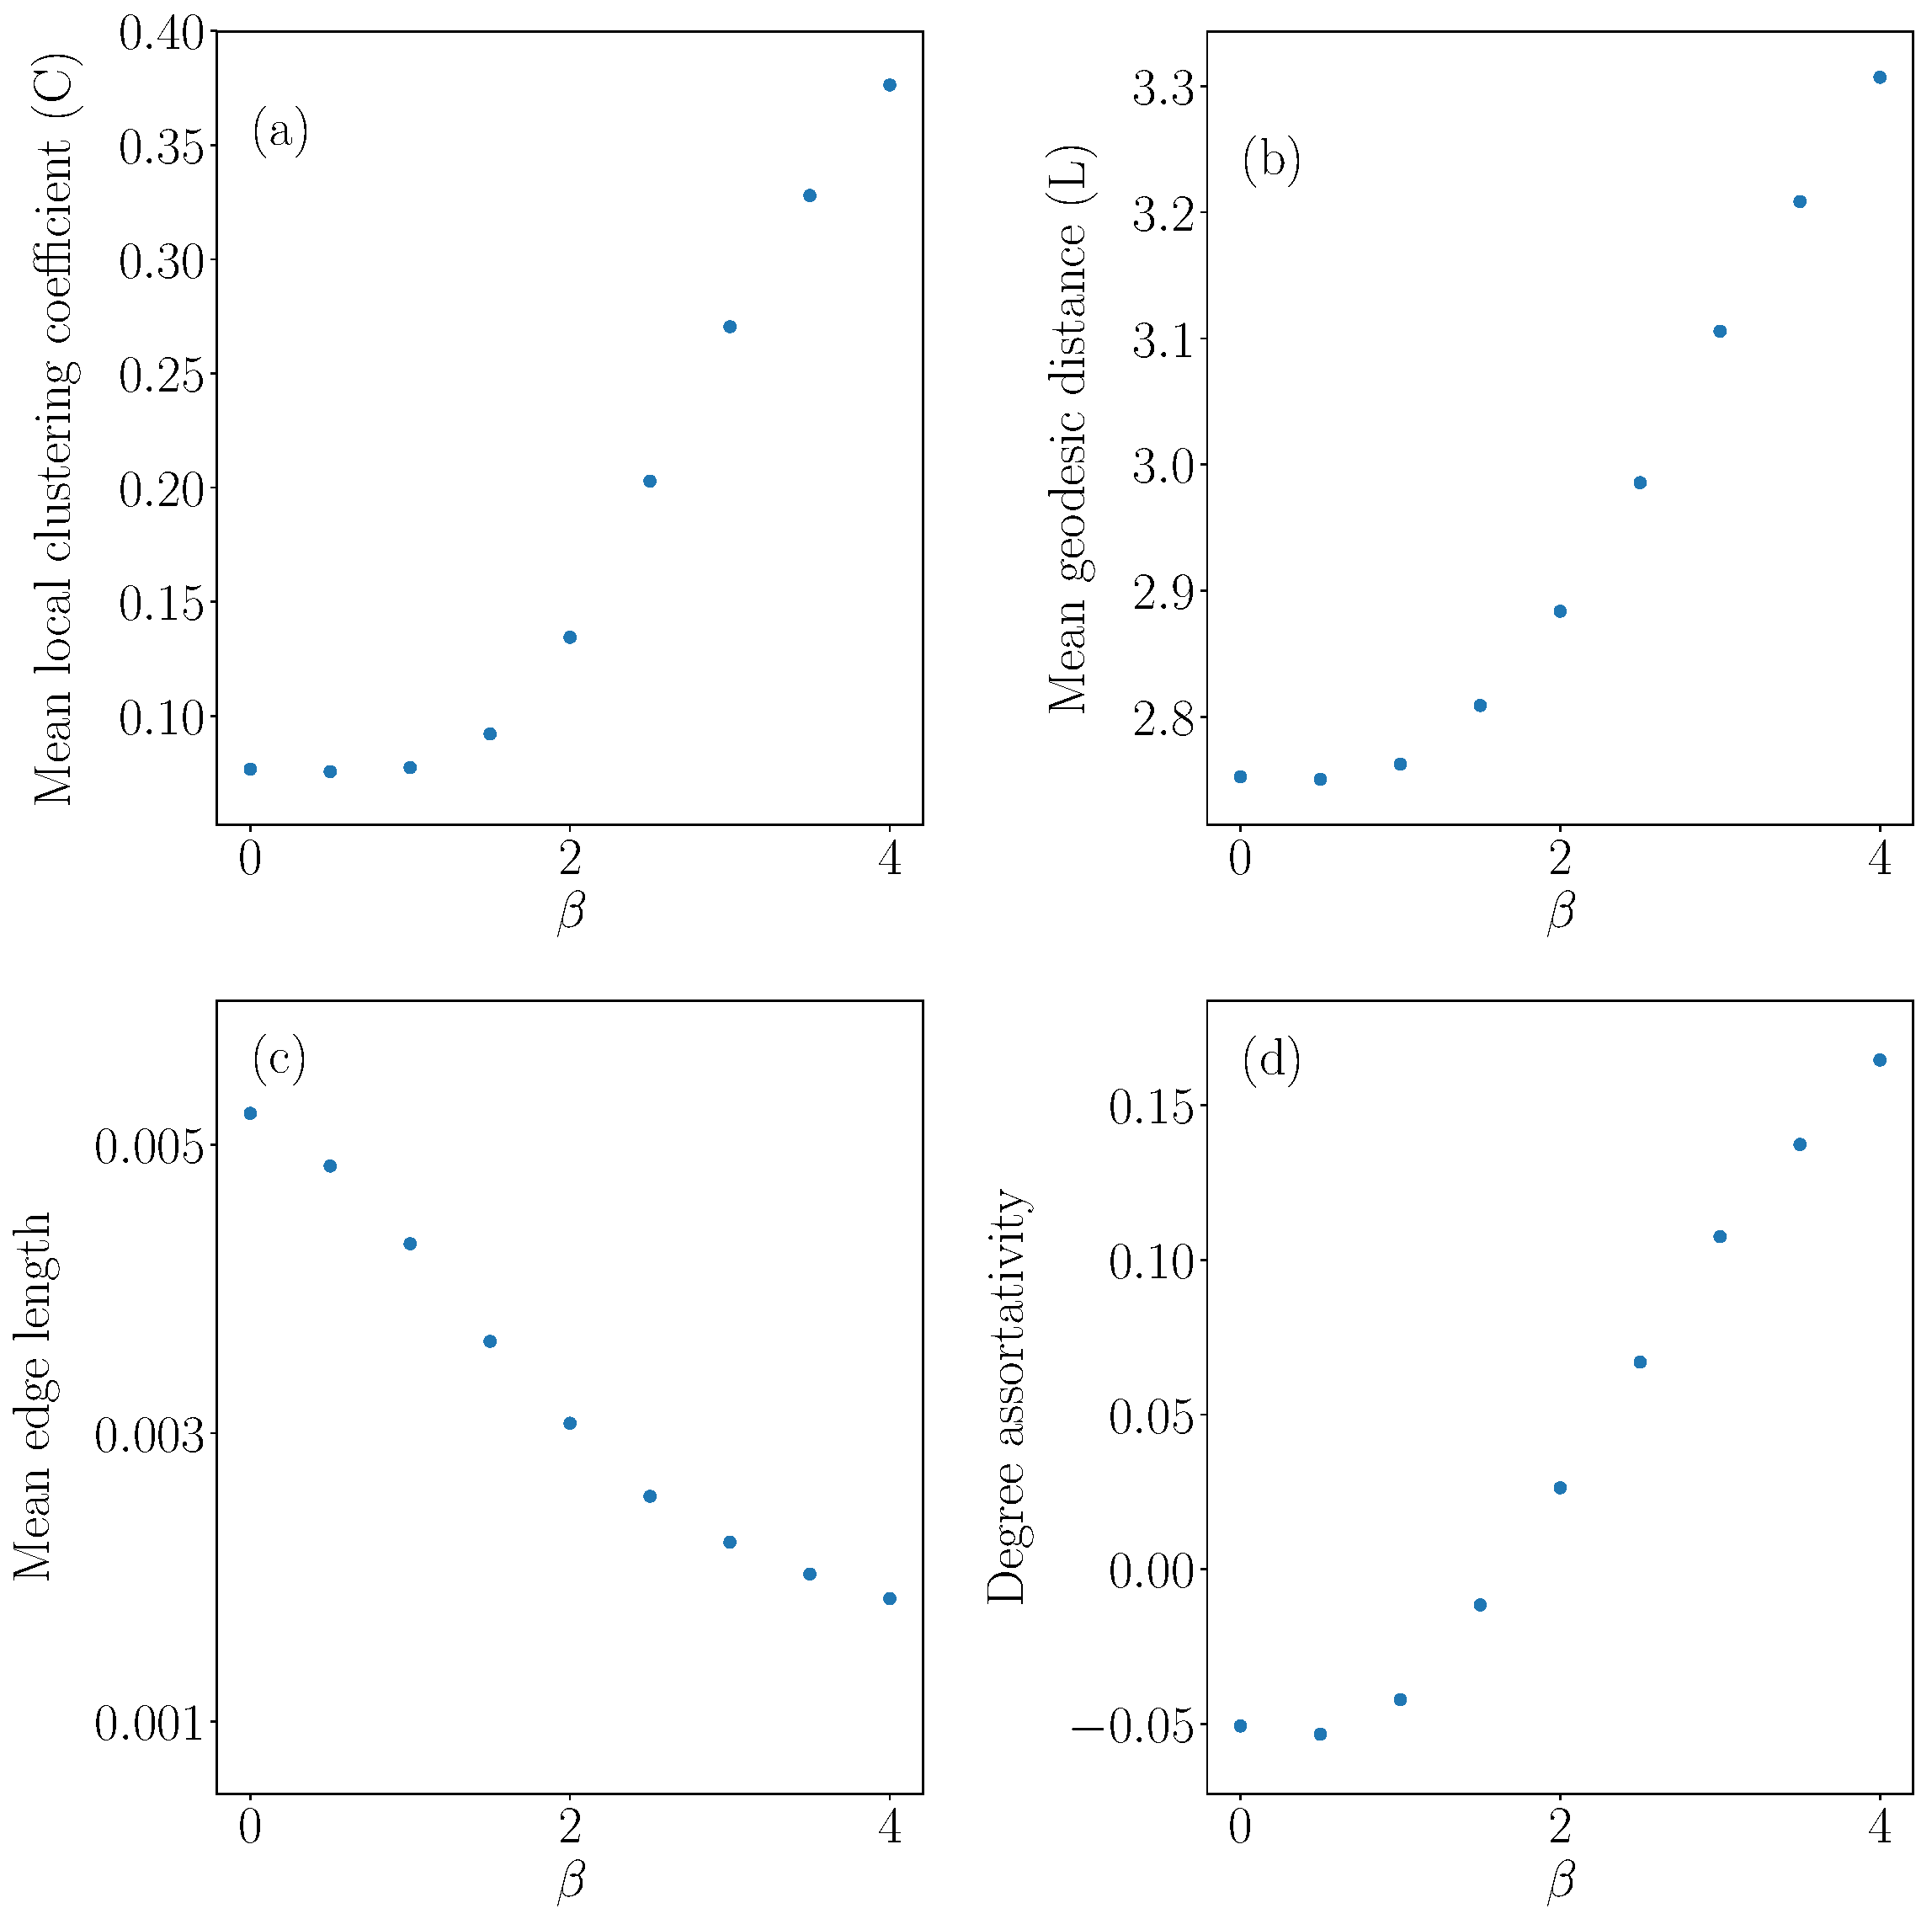
\includegraphics[width=0.65\linewidth]{../figures/preferential_attachment_metrics.pdf}
			\caption{Metrics for $n=10000$}
		\end{figure}
	}
	
	\frame {
		\frametitle{Network Models}
		\framesubtitle{SPA Characteristics}
		
\begin{columns}[onlytextwidth]
\begin{column}{.45\textwidth}
\begin{figure}
  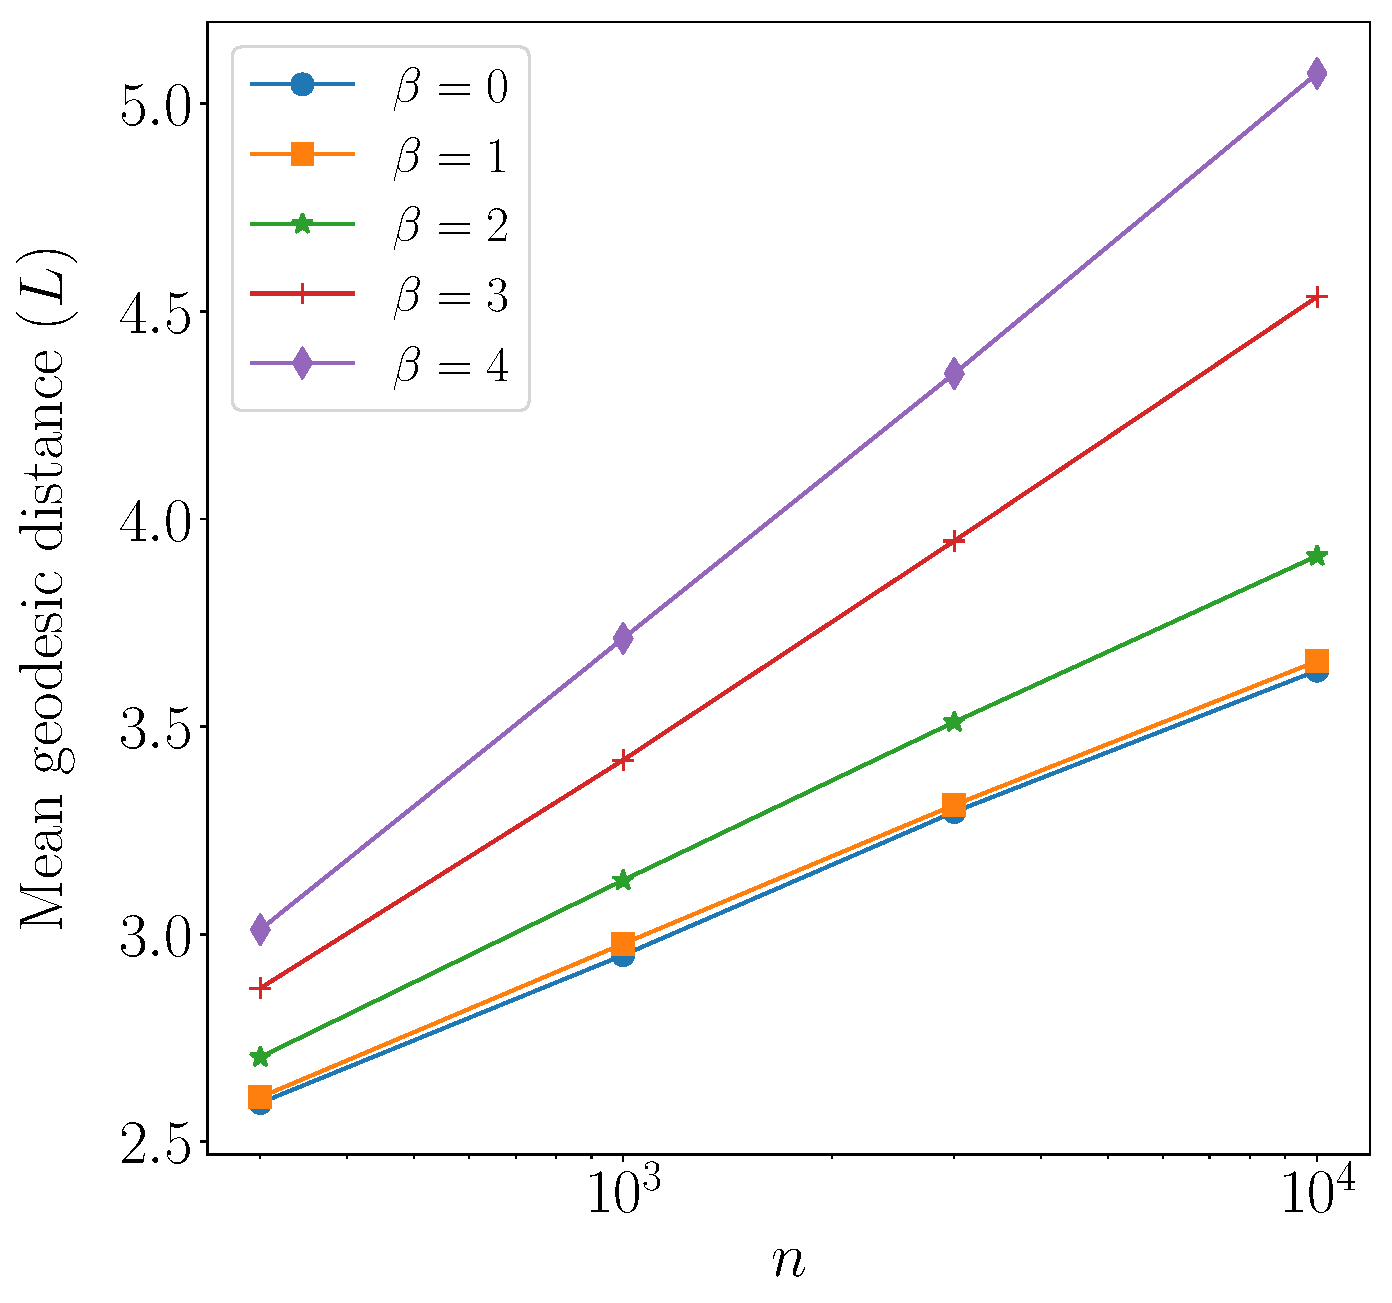
\includegraphics[width=\textwidth]{../figures/PA_log_geodesic.pdf}
  \caption{log-log $n$ vs. mean geodesic distance}
\end{figure}
\end{column}
\hfill
\begin{column}{.45\textwidth}
\begin{figure}
  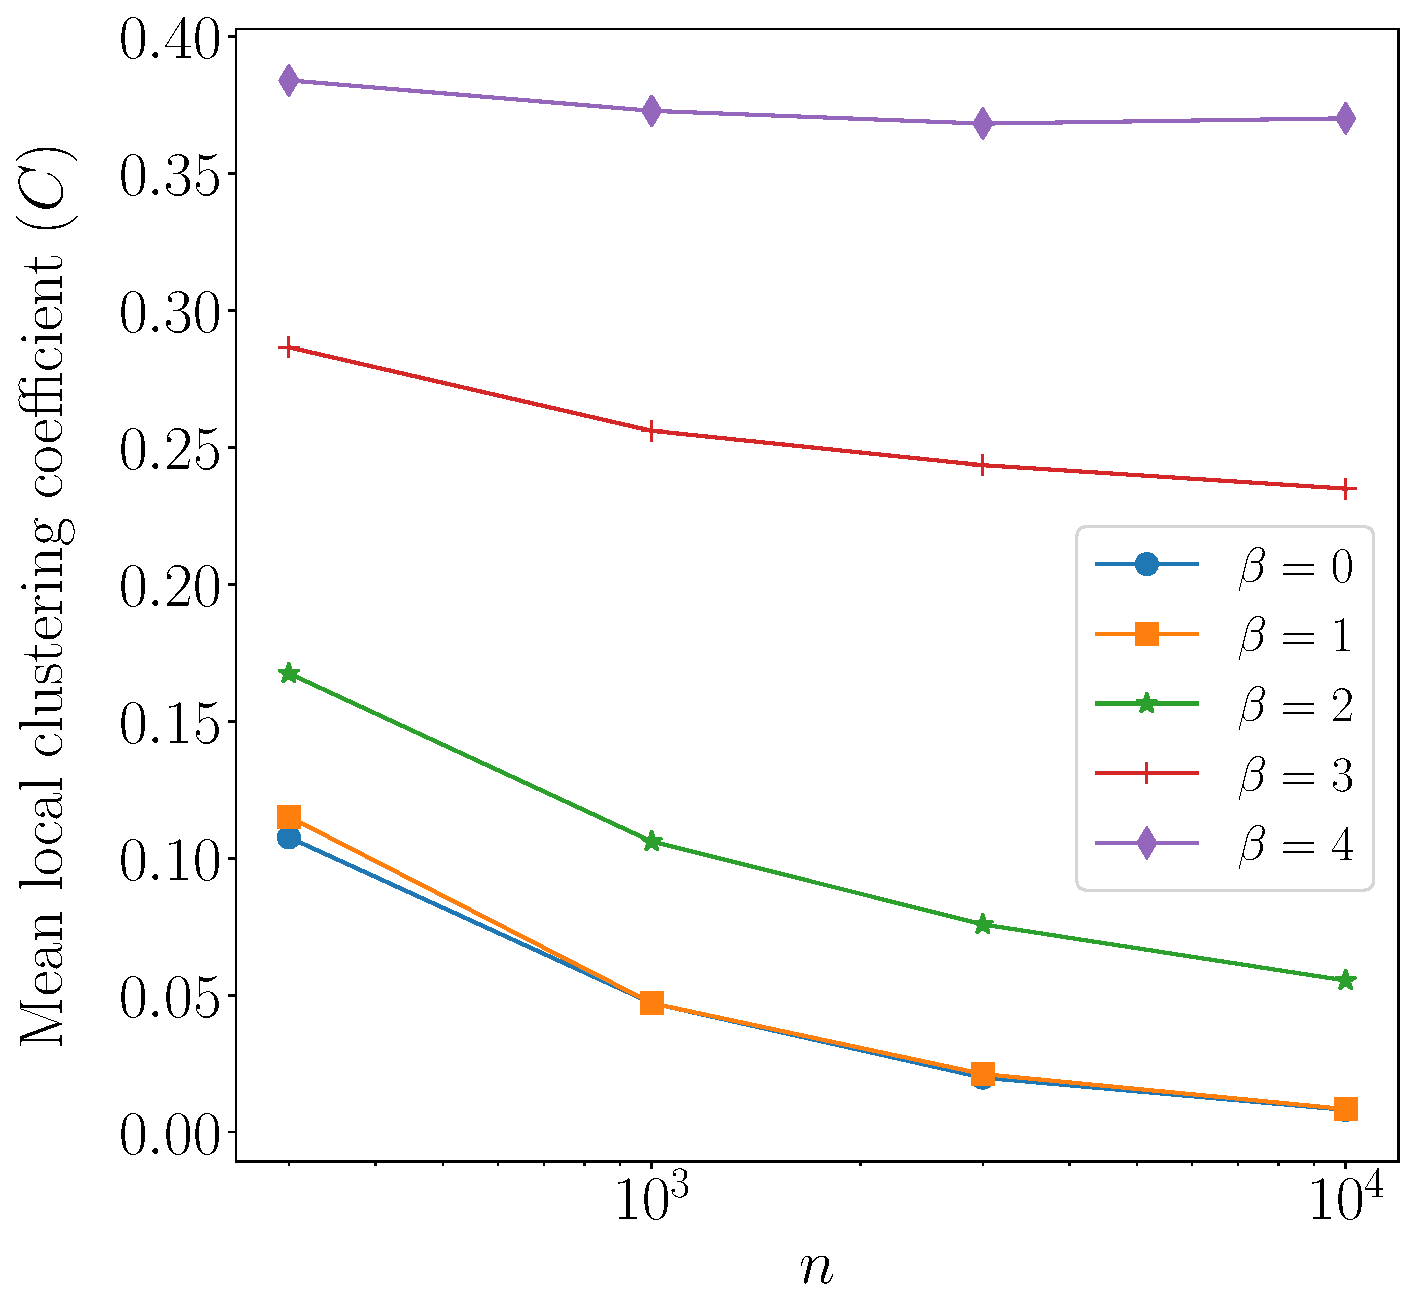
\includegraphics[width=\textwidth]{../figures/PA_log_clustering.pdf}
  \caption{log-log $n$ vs. clustering}
\end{figure}
\end{column}
\end{columns}		

		}
	
	
	
	%%%
	%%%
	
	
	
	\frame{
		\frametitle{Network Models 2}
		\framesubtitle{Inherent fitness model}
		Nodes have ``inherent fitness'' - propensity to gain edges
		
		\textbf{Model description:}
		\begin{itemize}
			\item $\bullet$ $n$ total nodes are each given a fitness value from a distribution, e.g. $f(w) = \lambda e^{-\lambda w}\,, \quad w \geq 0$
			\item $\bullet$ Each pair of nodes is considered and an edge formed between them depending on function $g$, e.g. Heavistep $g(v_i,v_j) = w_i + w_j \geq \theta$, $\theta$ threshold parameter
		\end{itemize}
		%some notable results - using an exponential distribution and heavistep to achieve powerlaw degree distribution, shown analytically
	}
	
	\frame{
	    \frametitle{Network Models 2}
	    \framesubtitle{Geographcial Fitness (GF) Model}
	    \textbf{Differences:}
	    \begin{itemize}
	    	\item $\bullet$ Network is embedded in $[0,1] \times [0,1]$ 2-dimensional space. Every new node is assigned a position uniformly at random
	    	\item $\bullet$ New probability of forming edges between pairs of nodes $g(v_i, v_j) = (w_i + w_j)h(r_{i,j}) \geq \theta$
	    \end{itemize}
	}

	\frame {
		\frametitle{Network Models 2}
		\framesubtitle{GF Model}
		Also consider using a different fitness distribution and edge forming probability:
				
		$$
		w_i \sim N(0, 1)
		$$
		$$
		g(v_i, v_j) = |w_i - w_j|h(r) \geq \theta
		$$
	}
	
	\frame {
		\frametitle{Network Models}
		\framesubtitle{GF Characteristics}
		%\begin{figure}
		%	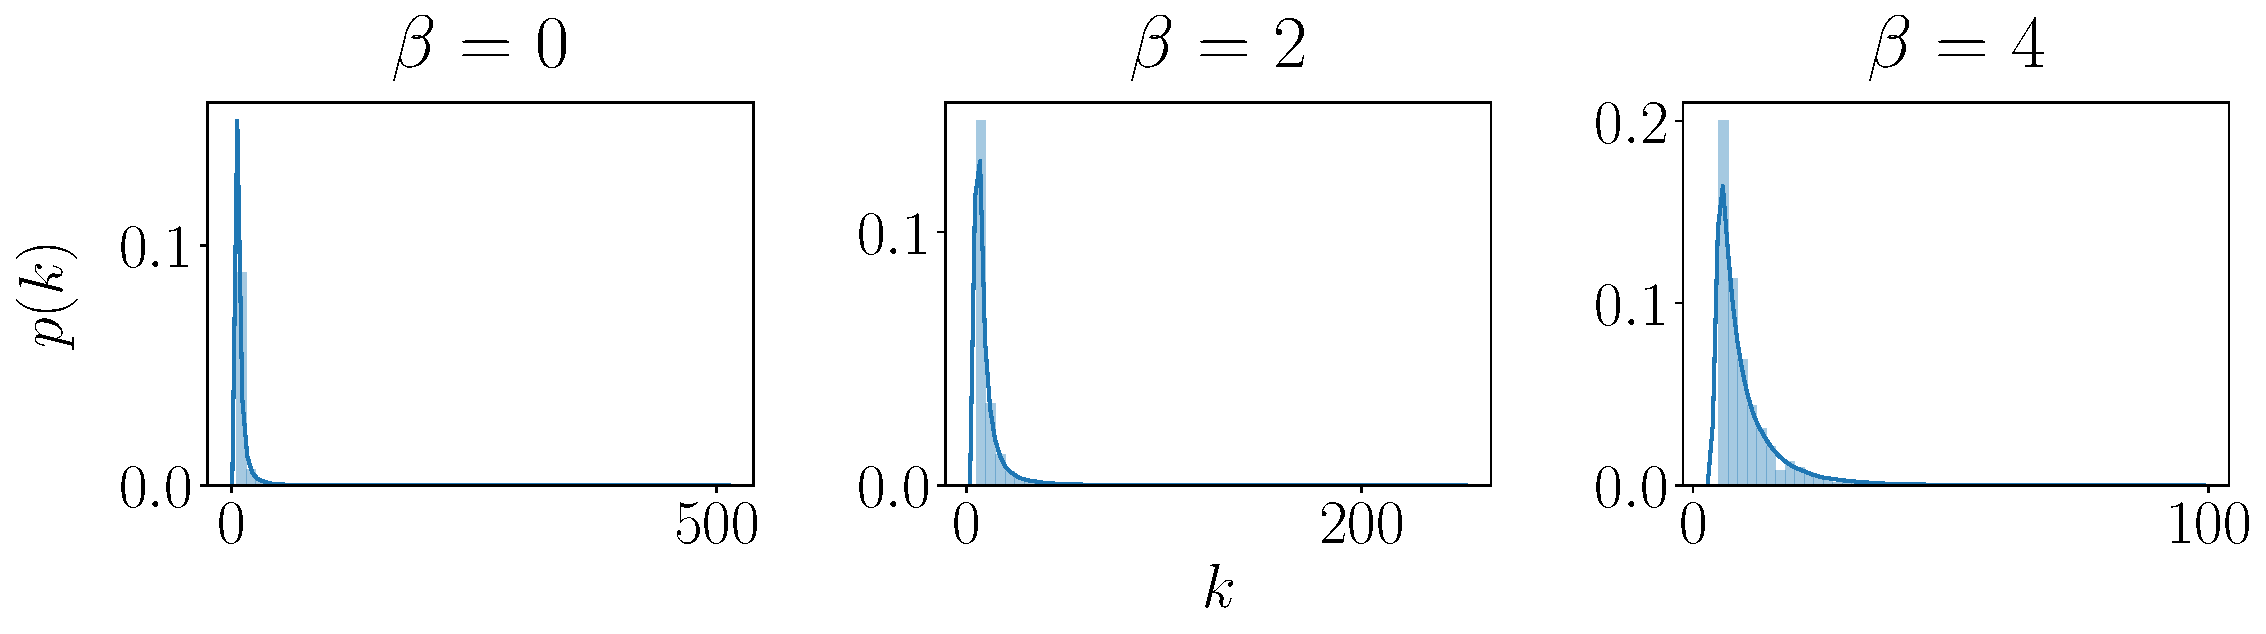
\includegraphics[width=0.5\linewidth]{../figures/preferential_attachment_degree_distribution.pdf}
		%	\caption{Degree distributions for $T=10000$}
		%\end{figure}
		
		\begin{figure}
			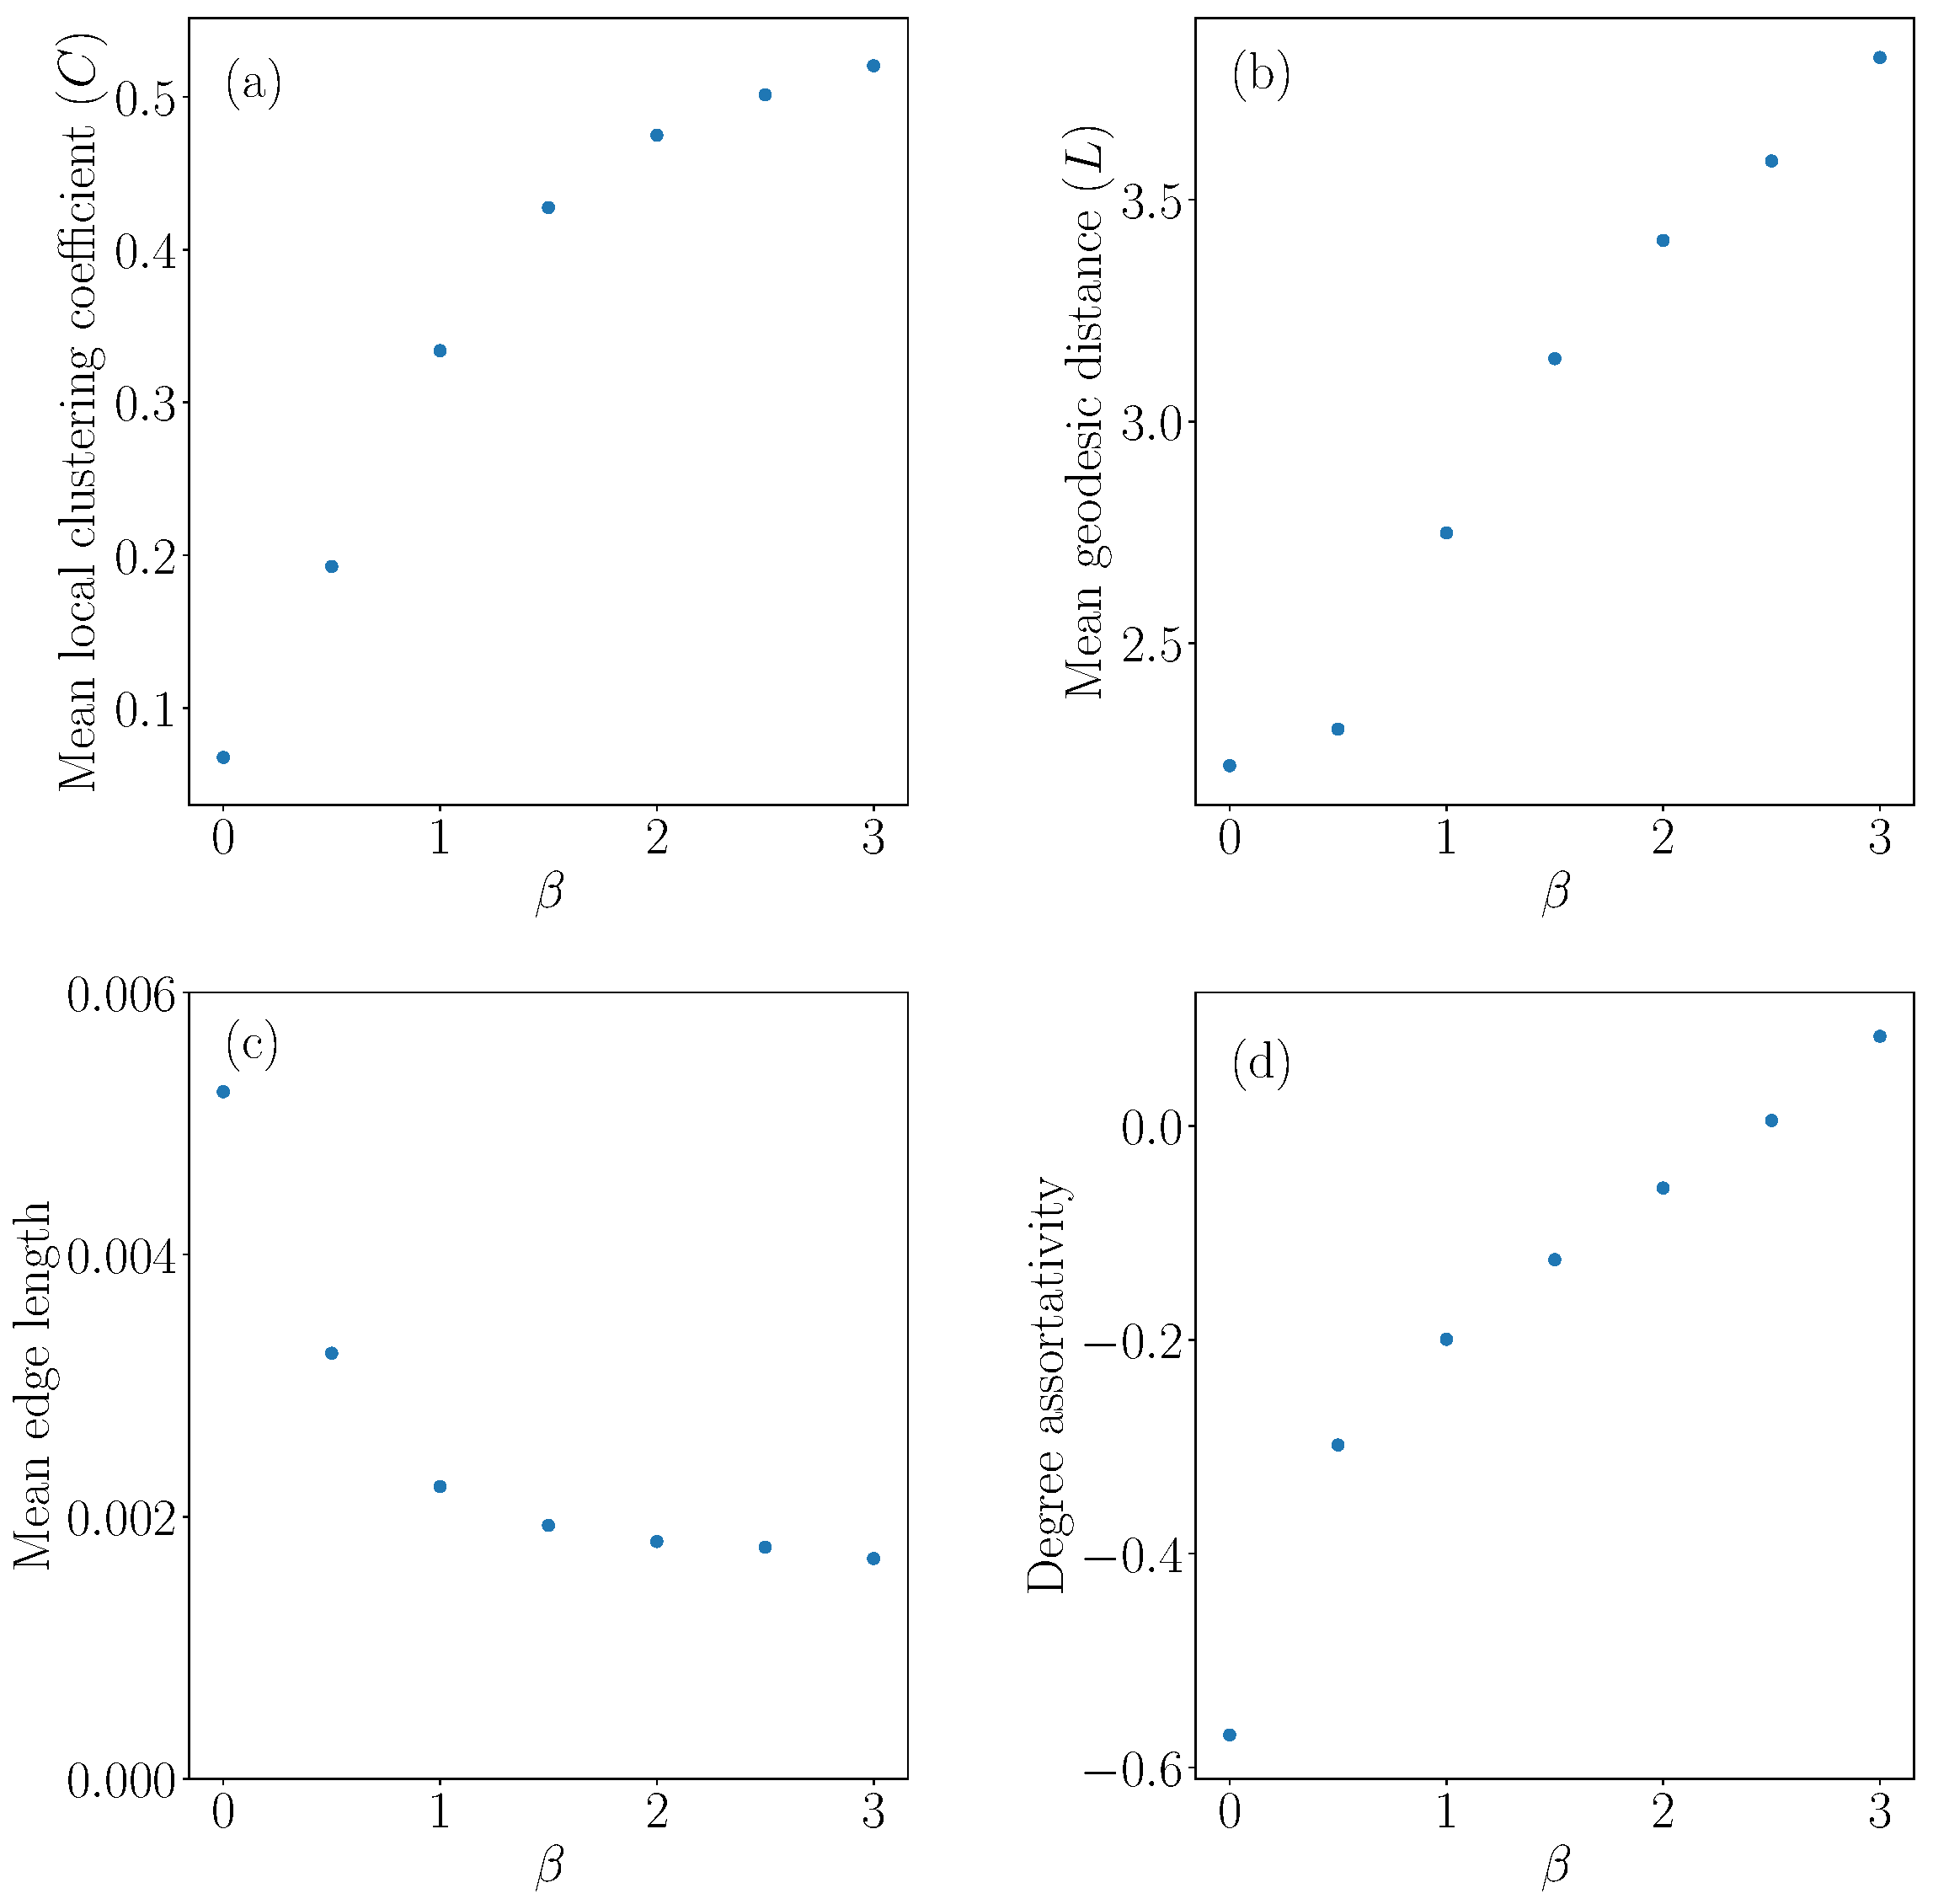
\includegraphics[width=0.65\linewidth]{../figures/geographical_network_metrics3.pdf}
		\end{figure}
	}
	
	\frame {
		\frametitle{Network Models}
		\framesubtitle{GF Characteristics}
		
		Closeness centrality:
		$$
		C(v_i) = \frac{n - 1}{\sum\limits_{i \neq j} d(v_i,v_j)}
		$$
		%$d(v_i, v_j)$ is the geodesic distance, closeness centrality measures how close a node is to all other nodes, so is a useful measure in quantifying how many shortcuts to other nodes there are
\begin{columns}[onlytextwidth]
\begin{column}{.4\textwidth}
\begin{figure}
  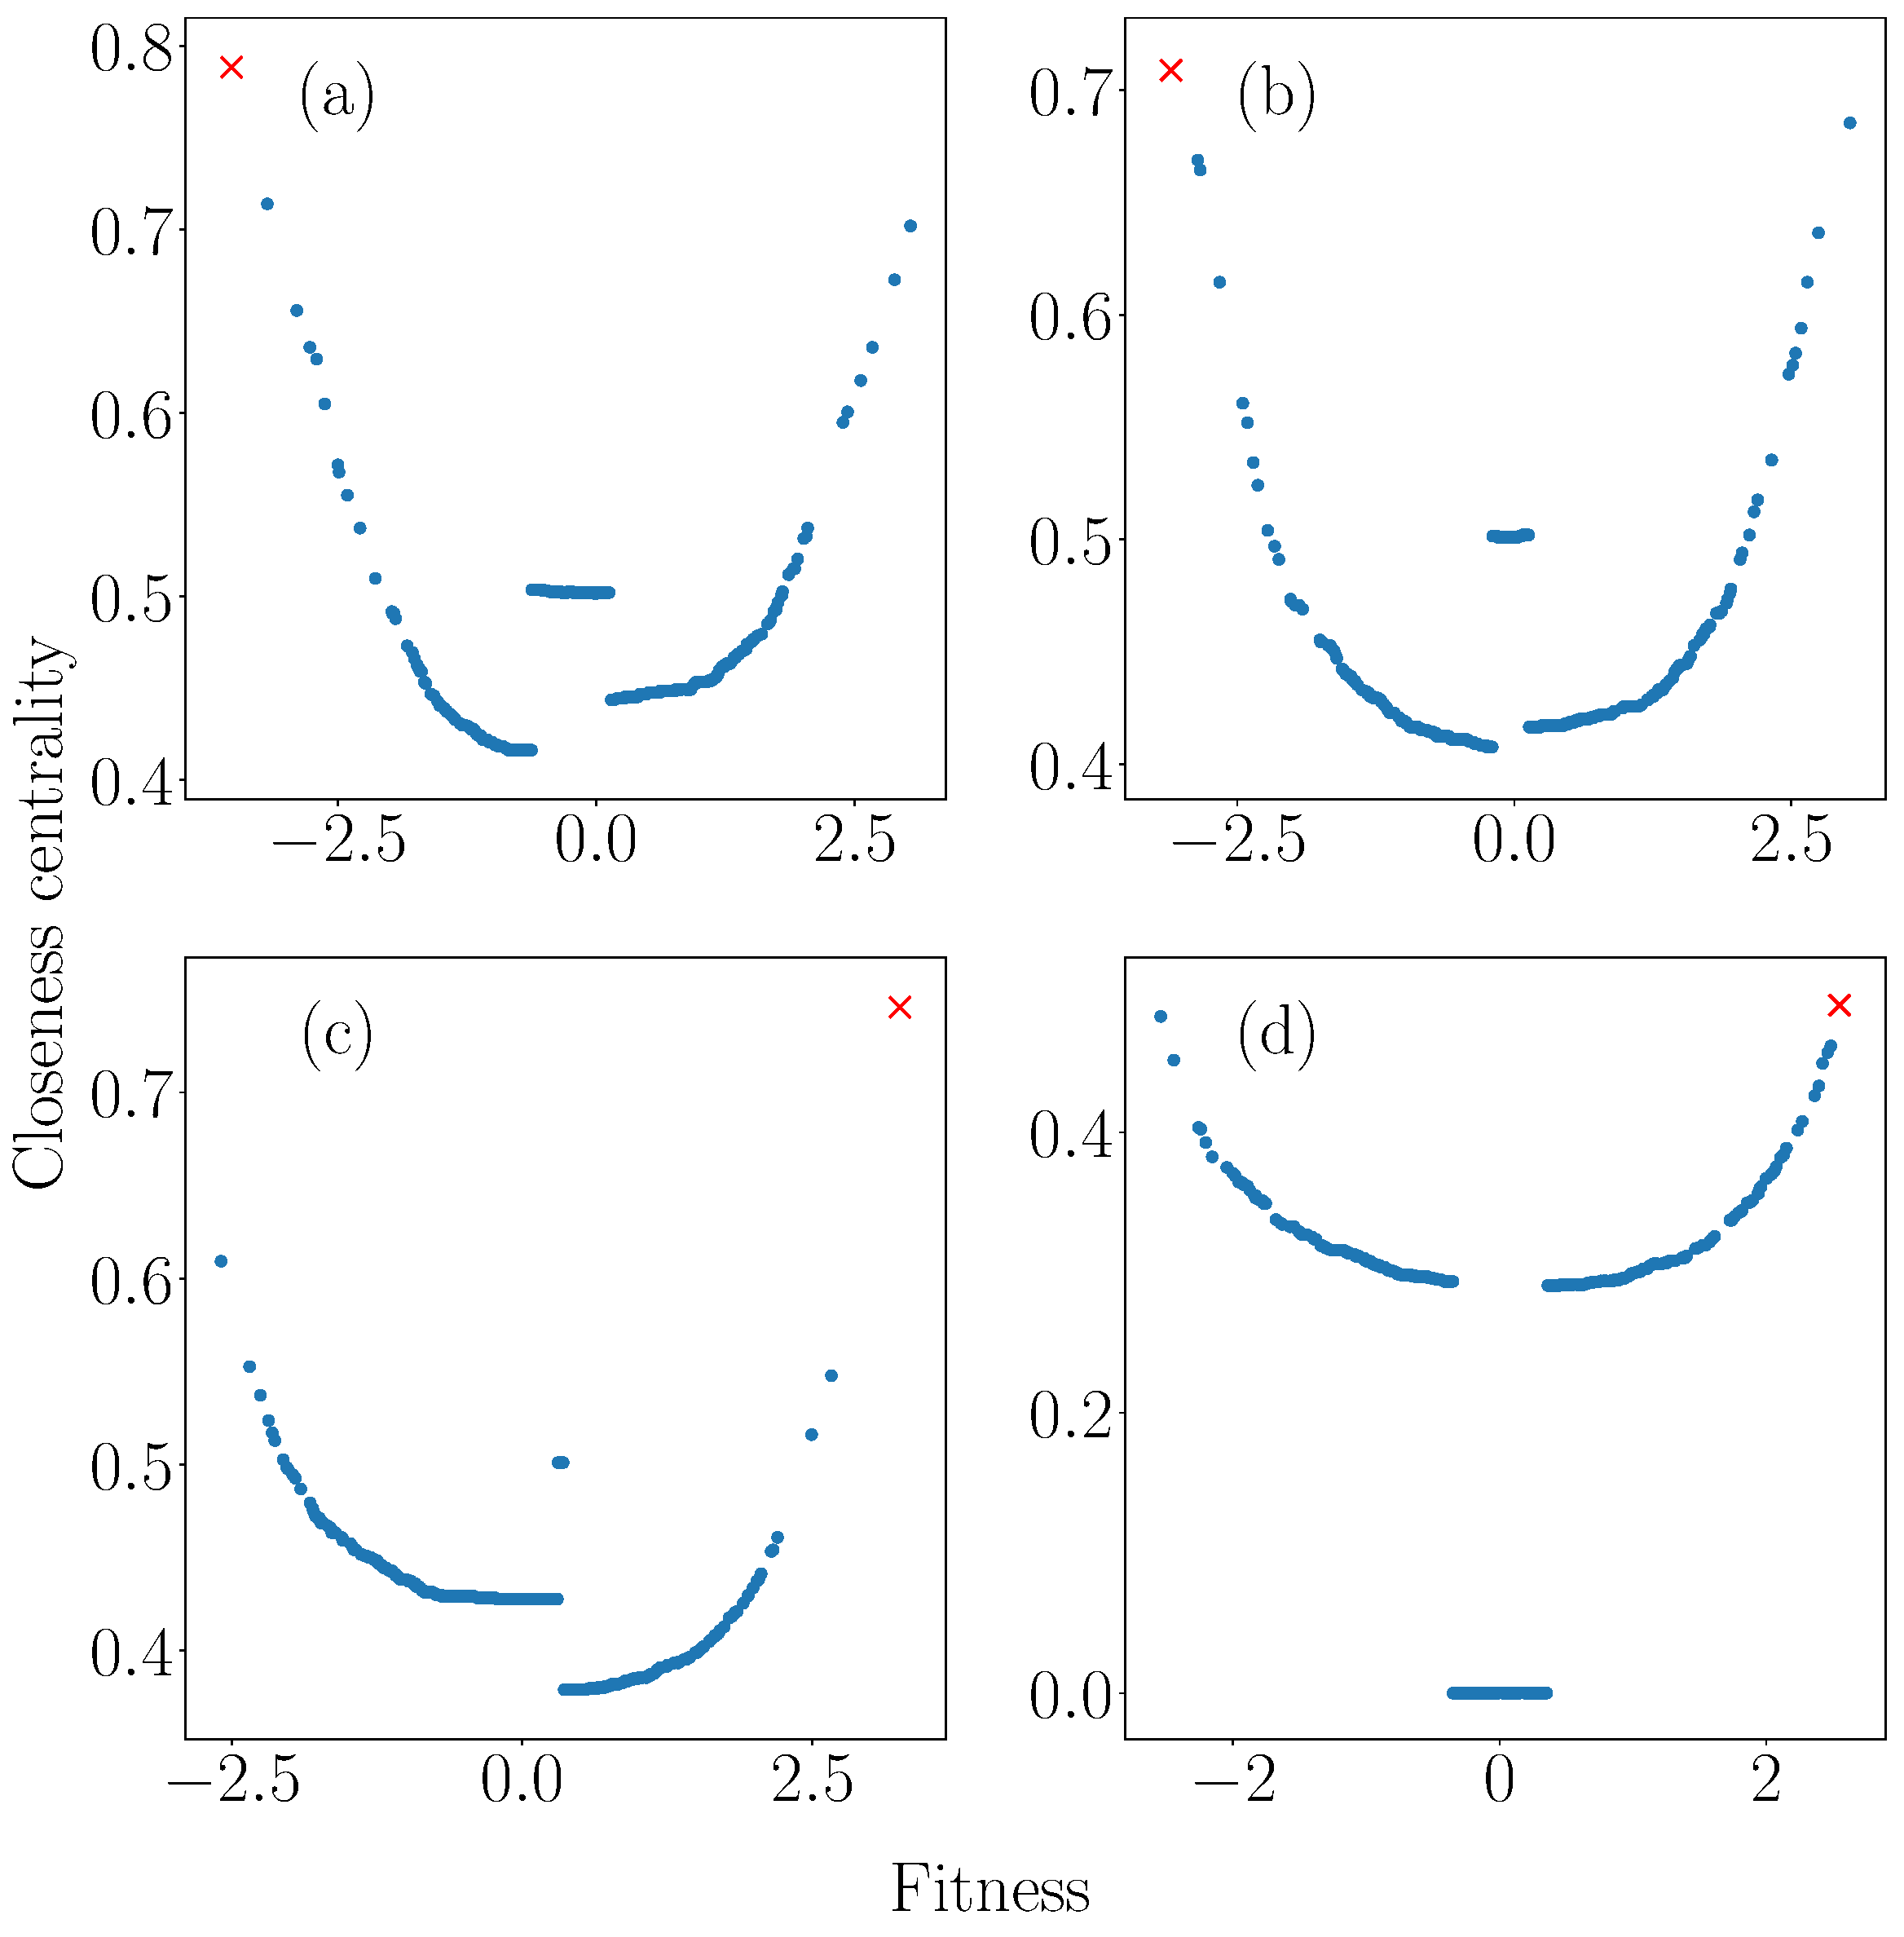
\includegraphics[width=\textwidth]{../figures/geographic_beta_0_examples2_largerfont.pdf}
  \caption{Closeness centrality for $\beta = 0$}
\end{figure}
\end{column}
\hfill
\begin{column}{.4\textwidth}
\begin{figure}
  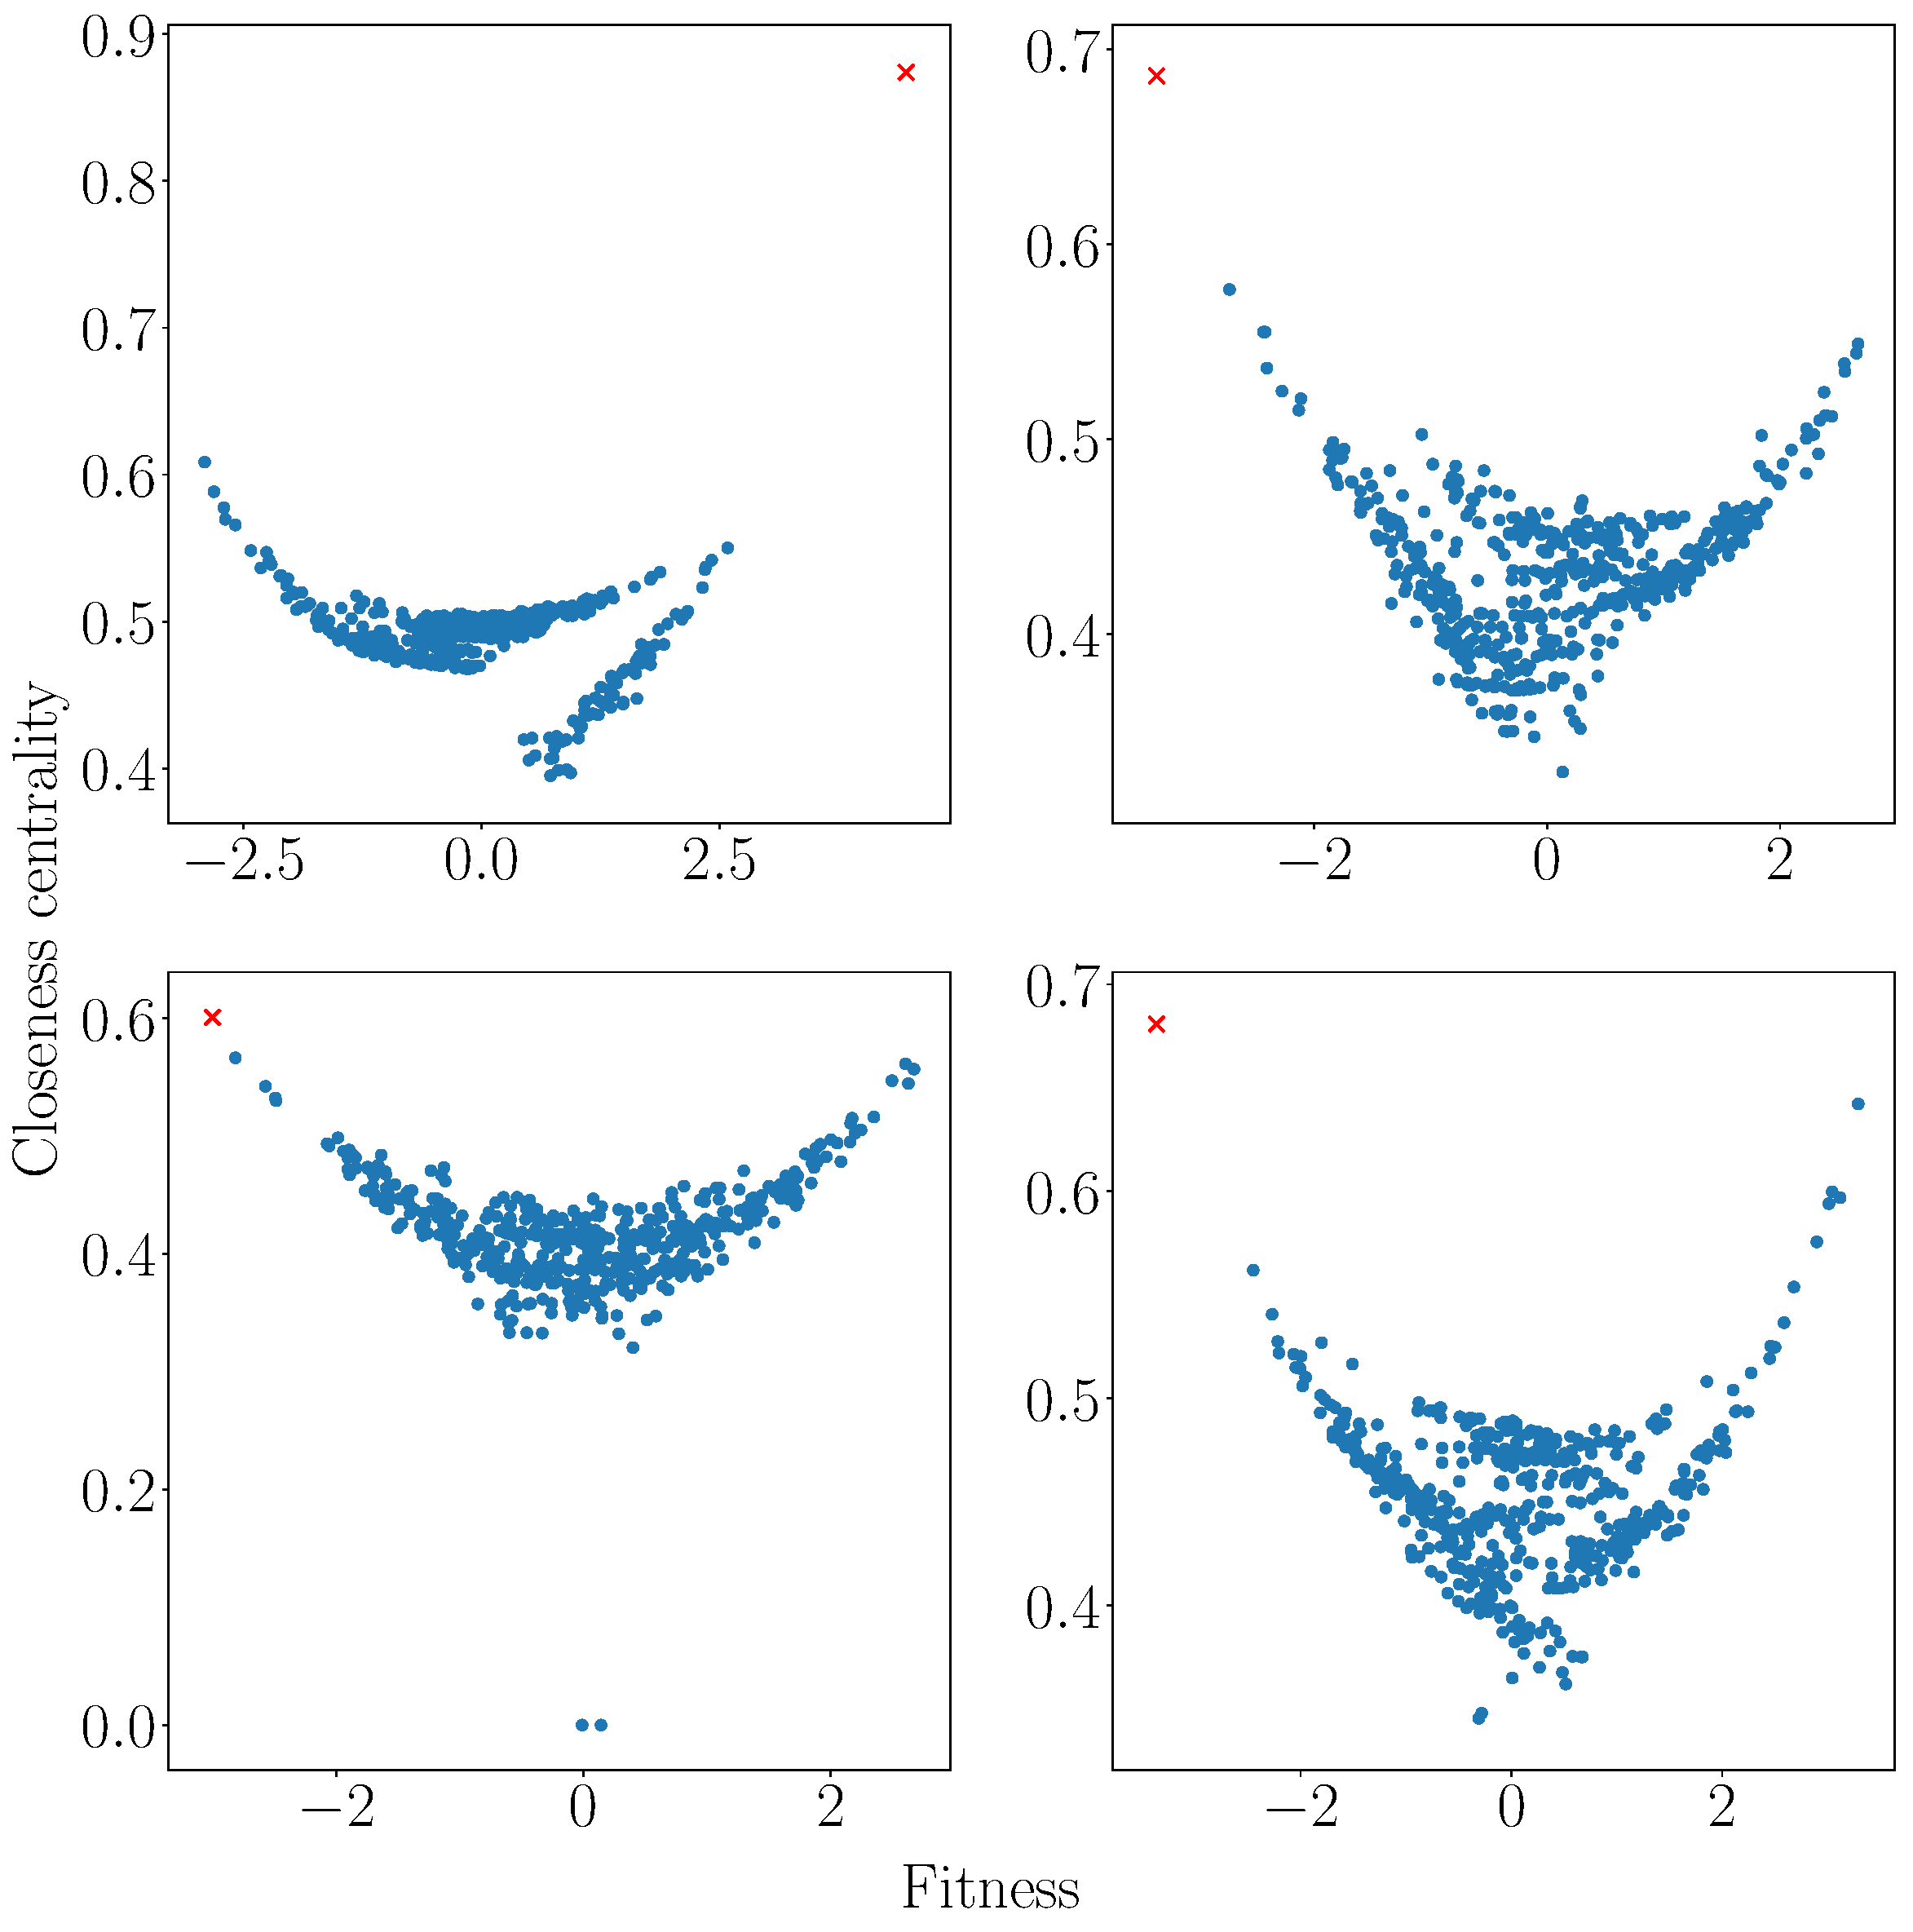
\includegraphics[width=\textwidth]{../figures/geographic_beta_05_examples_largerfont.pdf}
  \caption{Closeness centrality for $\beta = 0.5$}
\end{figure}
\end{column}
\end{columns}		

		}
	
	
	%%%
	%%%
	
	
	\frame{
		\frametitle{Network Models 3}
		\framesubtitle{Configuration Model}
		One of the most classic null models - preserve degree sequence
		
		\textbf{Model description:}
		\begin{itemize}
			\item $\bullet$ Fix a degree sequence (often taken from an existing network)
			\item $\bullet$ Assign edge stubs based on degree sequence, so each node is guaranteed to have 
			\item $\bullet$ Match edge stubs uniformly at random
		\end{itemize}		
		%some notable results - using an exponential distribution and heavistep to achieve powerlaw degree distribution, shown analytically
	}

	\frame{
		\frametitle{Network Models 3}
		\framesubtitle{Configuration Model}
		\begin{figure}
			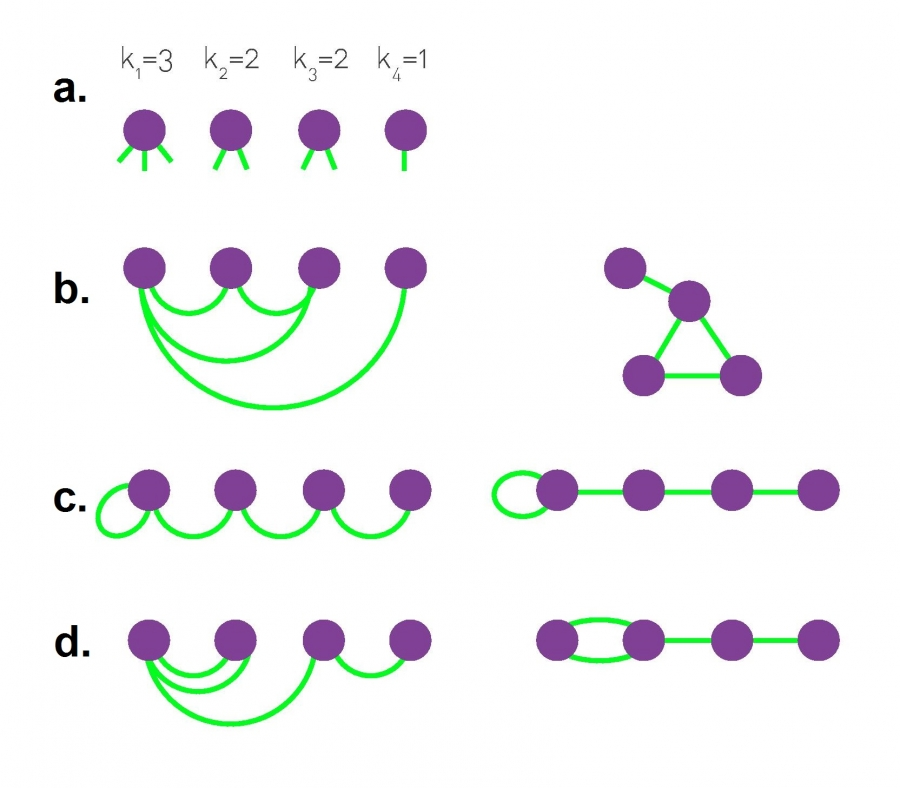
\includegraphics[width=0.7\linewidth]{degree_sequence_configuration.jpg}
			\caption{Taken from Albert-László Barabási - http://networksciencebook.com/}
		\end{figure}
	}
	
	\frame{
	    \frametitle{Network Models 3}
	    \framesubtitle{Spatial Configuration Model}
	    \textbf{Differences:}
	    \begin{itemize}
	    	\item $\bullet$ $n$ nodes given random location in $[0, 1] \times [0, 1]$ with stubs from degree sequence
	    	\item $\bullet$ Stub matching is proportional to distance from nodes, i.e.
	    	$$
	    	p(v_i, v_j, t) = \frac{u(v_j, t)h(r_{i,j})}{\sum_{l \neq i} u(v_l, t)h(r_{i,l})}
	    	$$
	    	where $u(v_j, t)$ is the number of stubs that $v_j$ has at time $t$
	    \end{itemize}
	}
	
	\frame {
		\frametitle{Network Models 3}
		\framesubtitle{Spatial Configuration Characteristics}
		%\begin{figure}
		%	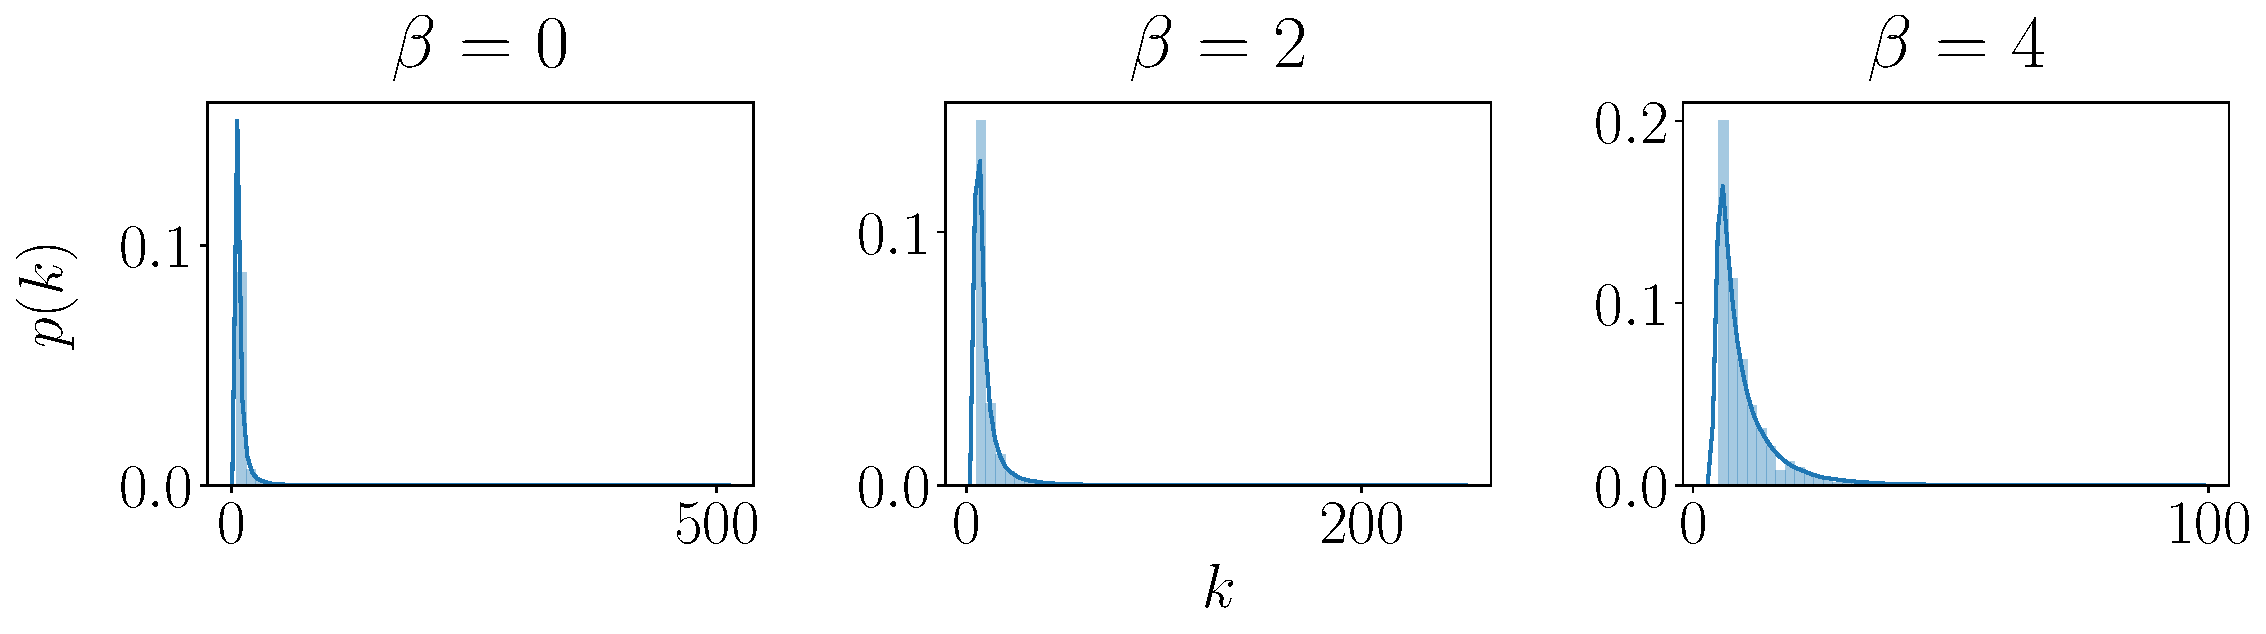
\includegraphics[width=0.5\linewidth]{../figures/preferential_attachment_degree_distribution.pdf}
		%	\caption{Degree distributions for $T=10000$}
		%\end{figure}
		
		\begin{figure}
			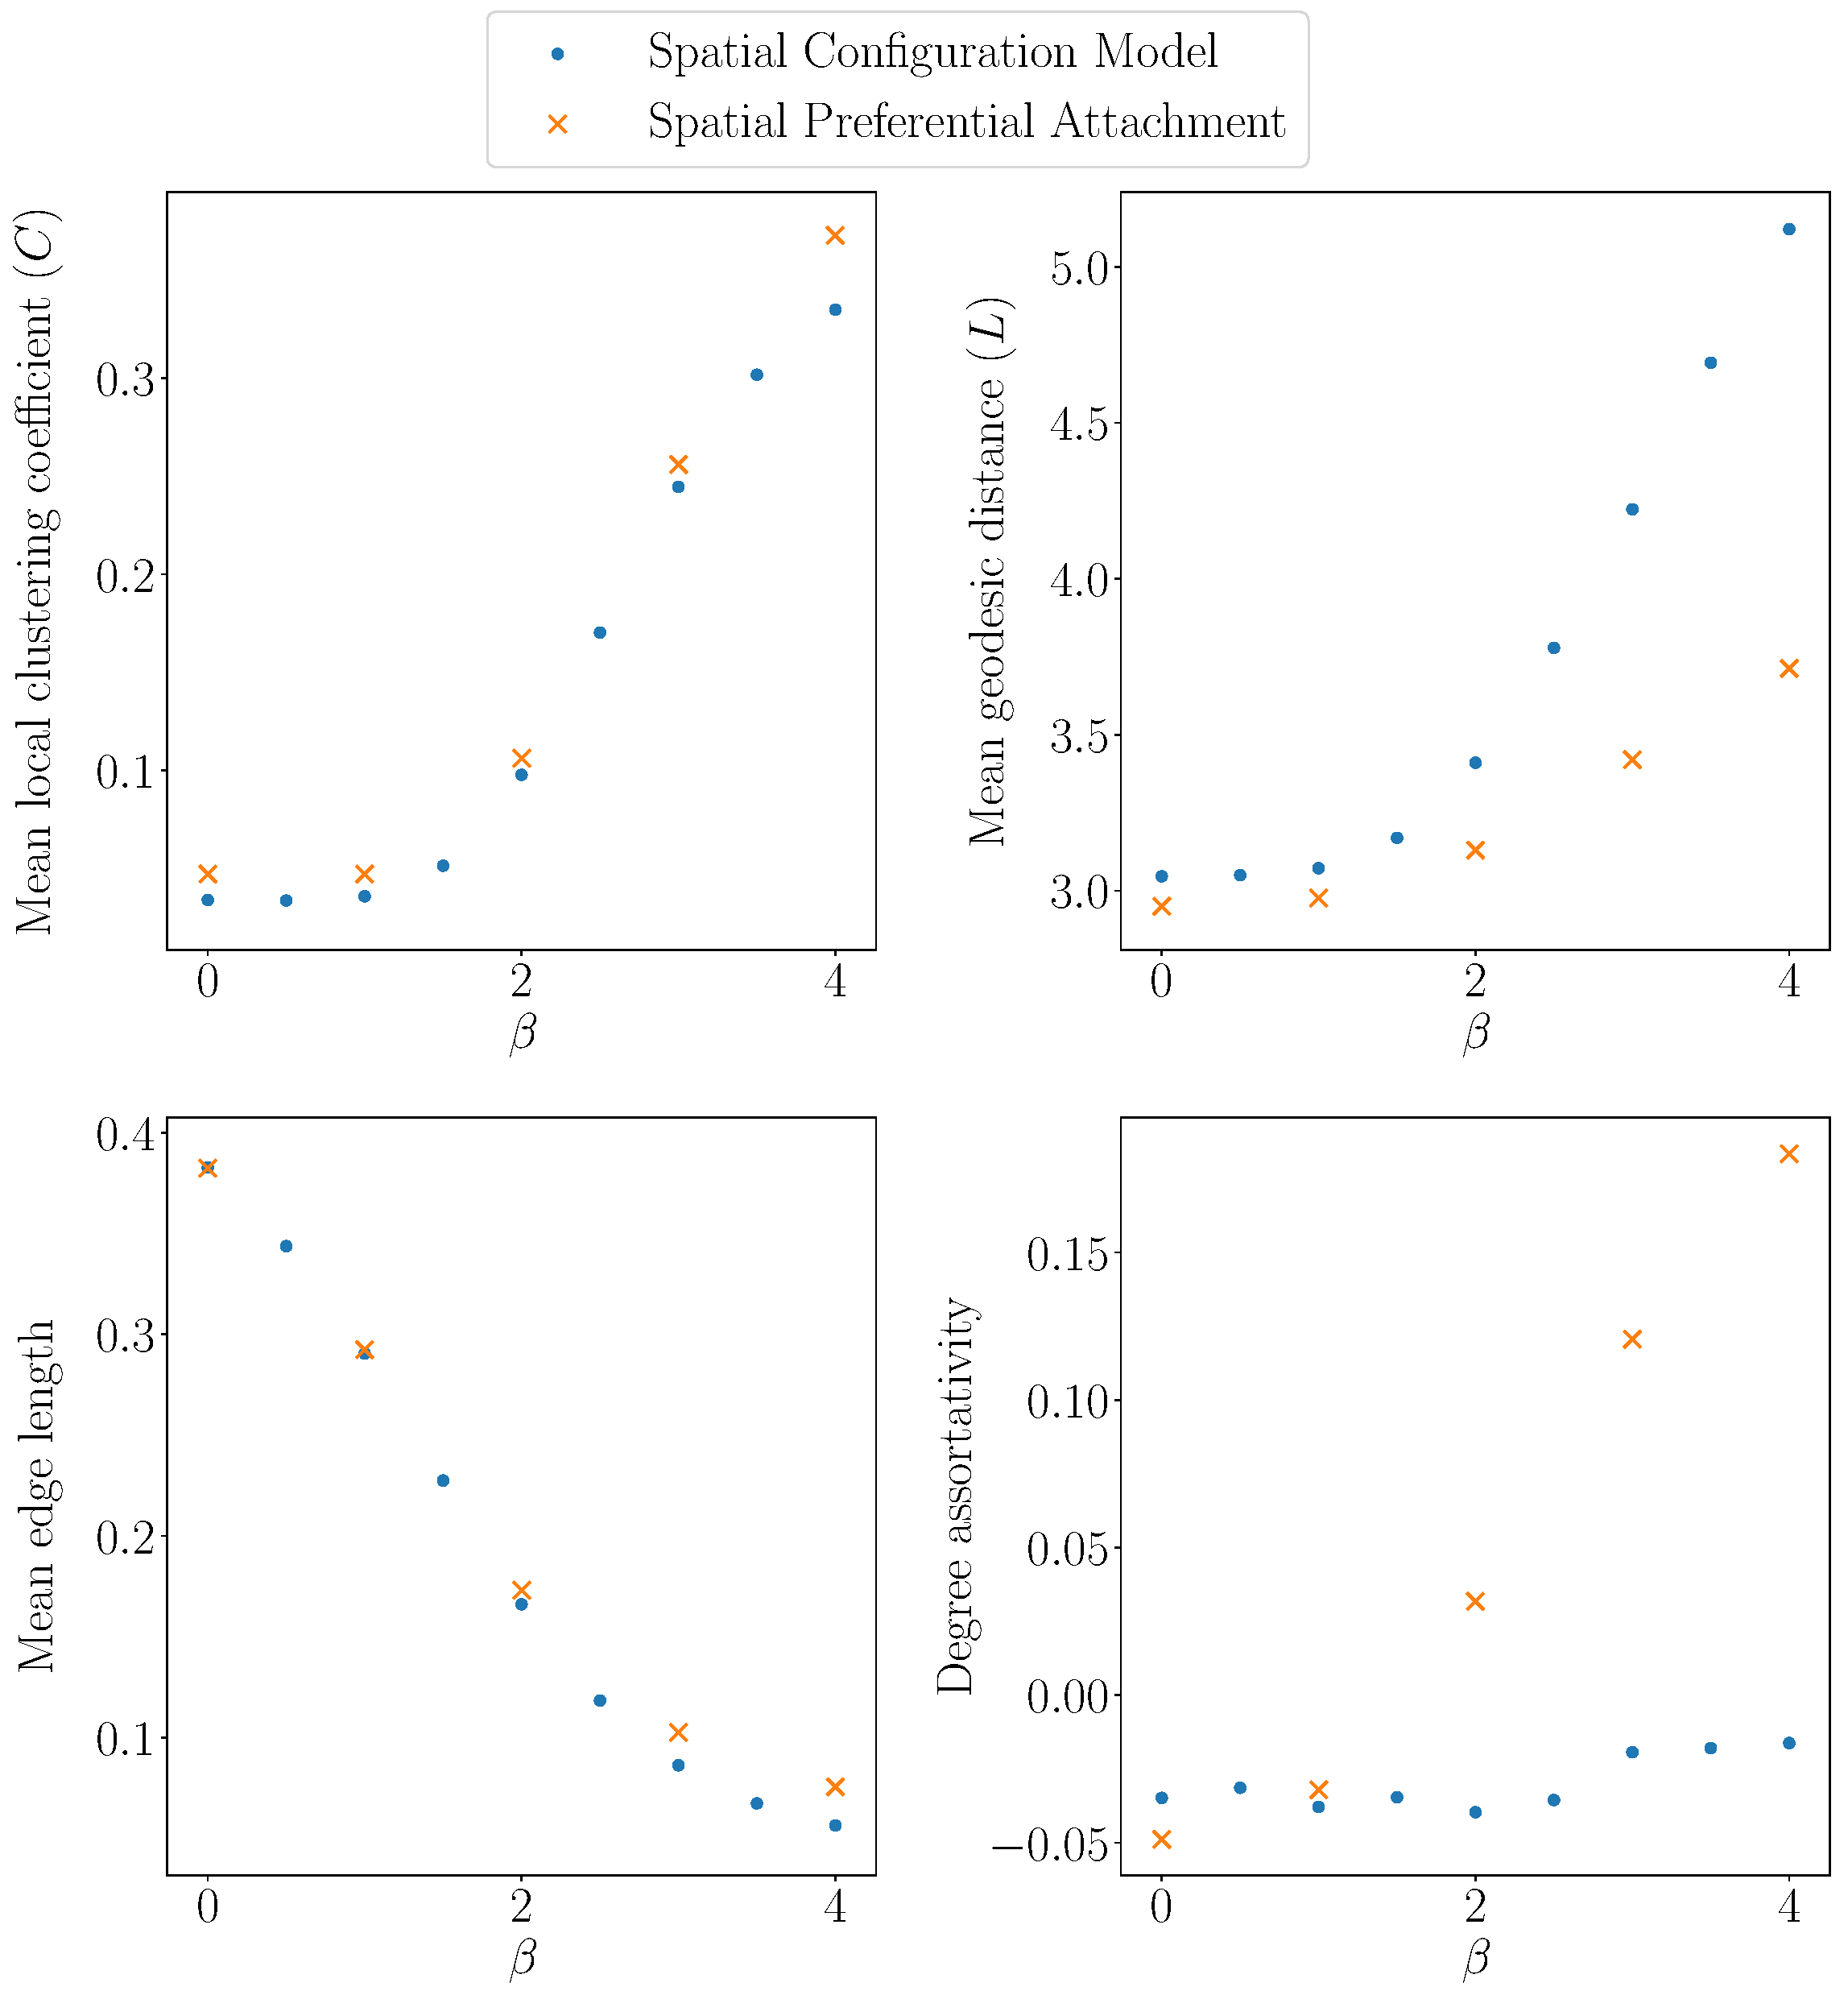
\includegraphics[width=0.65\linewidth]{../figures/spatial_preferential_comparison.pdf}
		\end{figure}
	}

	\frame {
		\frametitle{Network Models 3}
		\framesubtitle{Concluding Thoughts}
		Generally spatial models may be useful as null models or for creating families of networks to model systems
		
		As $\beta$ increases, the importance of distances between nodes increases, but can we quantify this?
		
	}
	
	
	
	%%%
	%%%
	
	
	
	\frame {
		\frametitle{Spatial Strength}
		\framesubtitle{Idea}
		
		Quantity to measure ``how strongly spatial embedding effects network structure''
		
		Idea: have a centrality that captures whether nodes are adjacent due to spatial embedding, or due to other network structure reasons
	}
	
	\frame {
		\frametitle{Spatial Strength}
		\framesubtitle{Definition}
		$N(v_i)$ is the neighborhood of $v_i$, then\\
		
		Normalized mean edge length:
		$$L(v_i) = \frac{\sum_{v_j \in N(v_i)}r_{i,j}}{k_i} \frac{1}{{\langle L \rangle}}$$
		
		Mean neighbor degree:
		$$ K(v_i) = \frac{\sum_{v_j \in N(v_i)} k_j}{k_i} \frac{1}{\langle k \rangle}
		$$
		
		Finally, spatial strength centrality:
		$$S(v_i) := \frac{1}{L(v_i)K(v_i)}
		$$
	}
	
	\frame {
		\frametitle{Spatial Strength}
		\framesubtitle{Spatial strength of models}
		\begin{figure}
			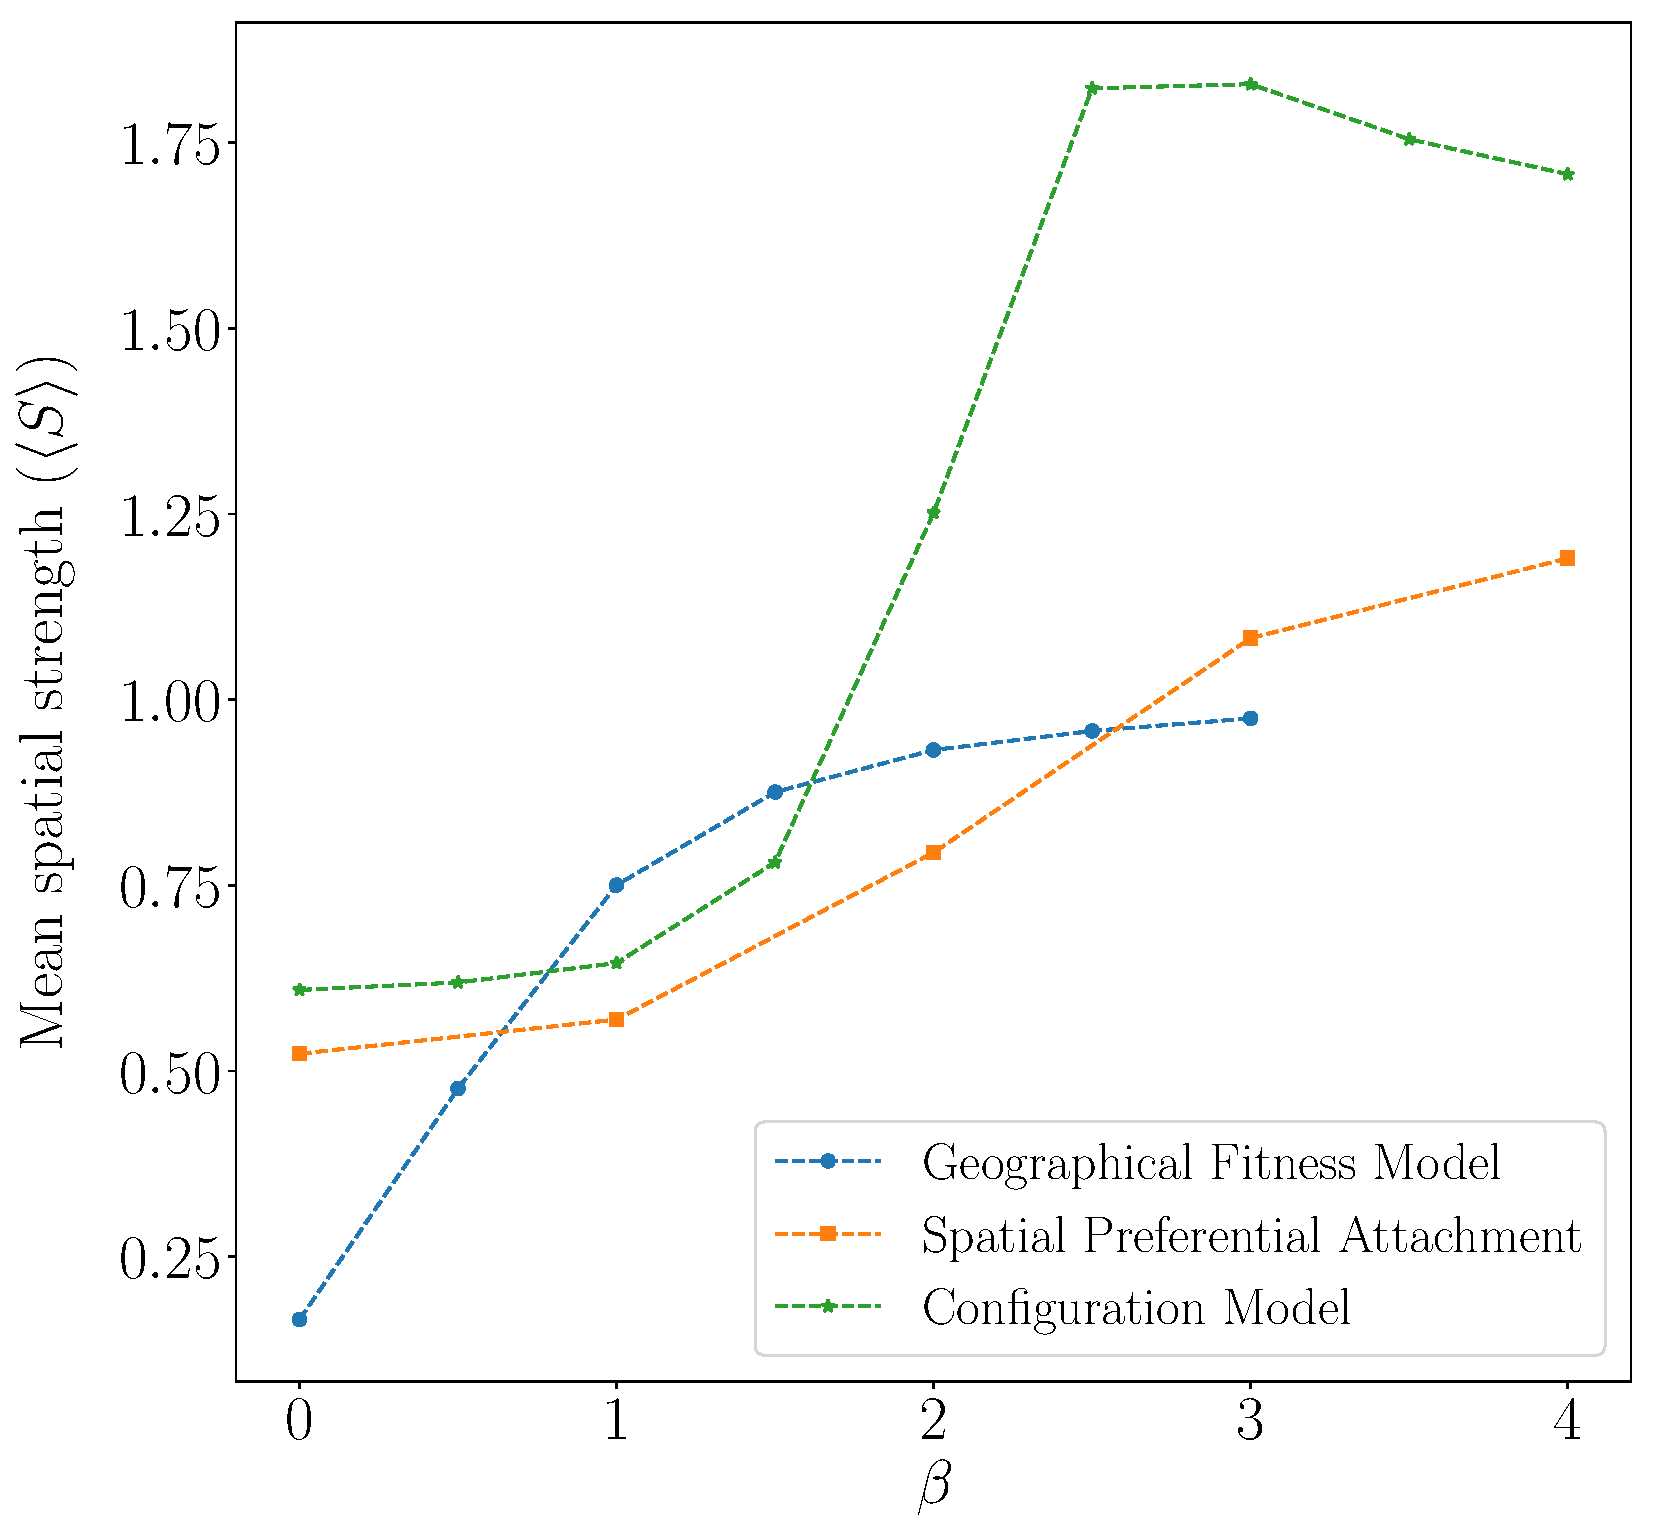
\includegraphics[width=0.65\linewidth]{../figures/spatial_model_spatial_strengths2.pdf}
		\end{figure}
	}
	
	\frame {
		\frametitle{Spatial Strength}
		\framesubtitle{Visual examples}
		\begin{figure}
			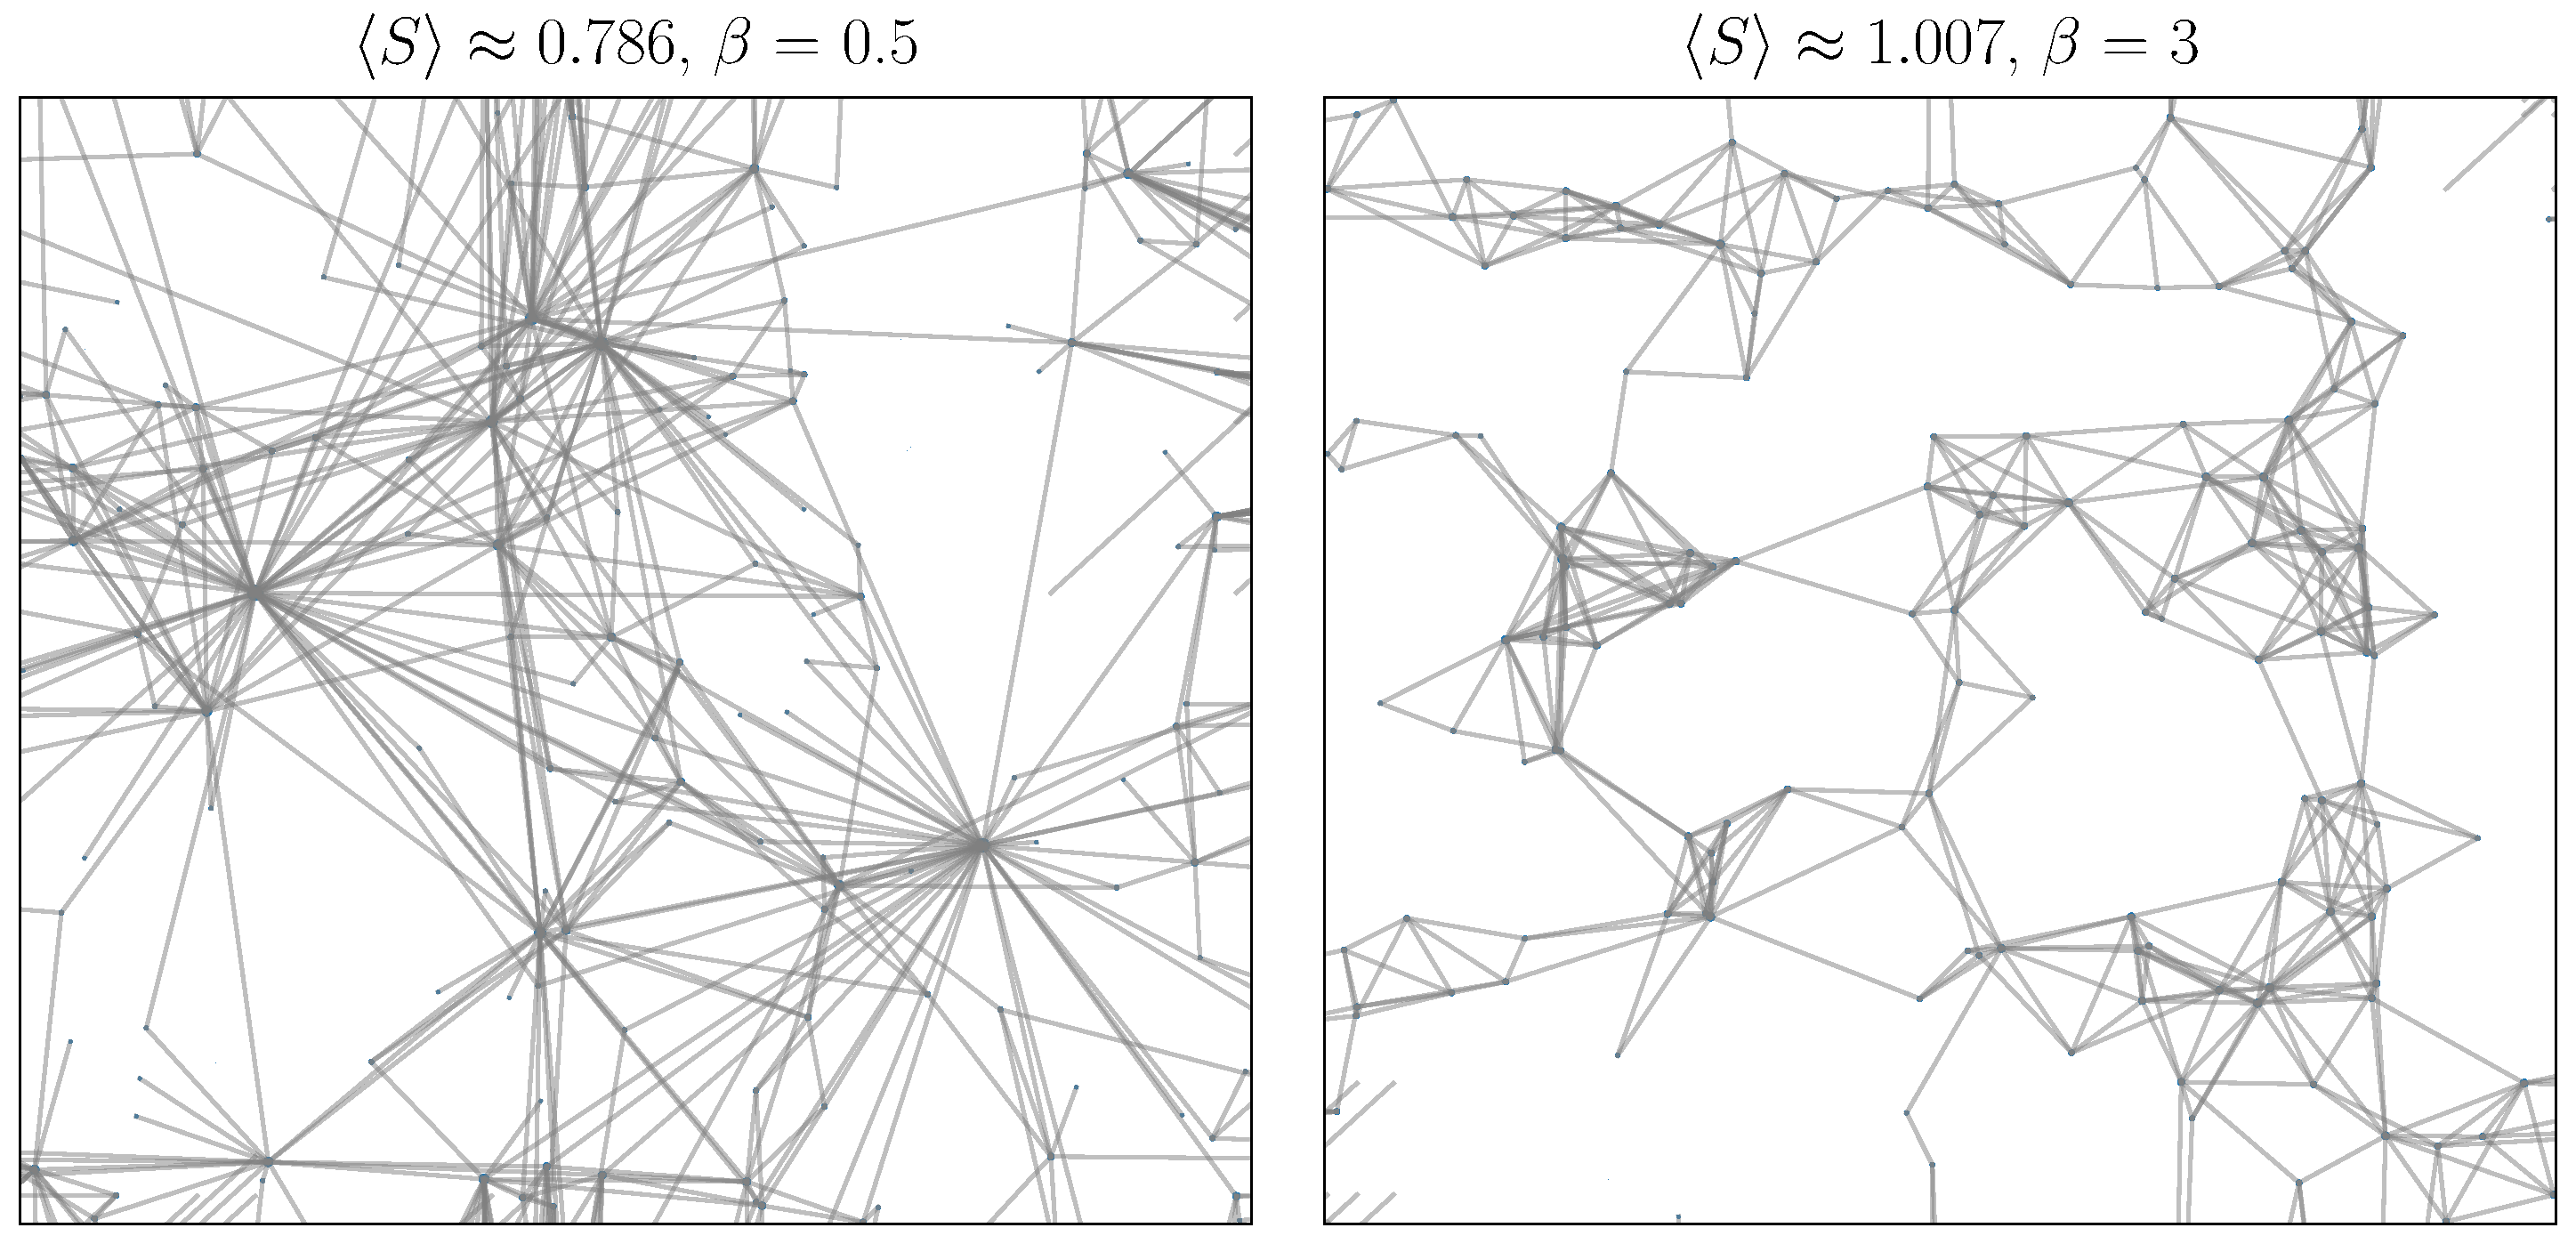
\includegraphics[width=0.9\linewidth]{../figures/geographic_example_no_highlight2horiz.pdf}
			\caption{Examples for GF model}
		\end{figure}
	}
	
	\frame {
		\frametitle{Spatial Strength}
		\framesubtitle{Visual examples 2}
		\begin{figure}
			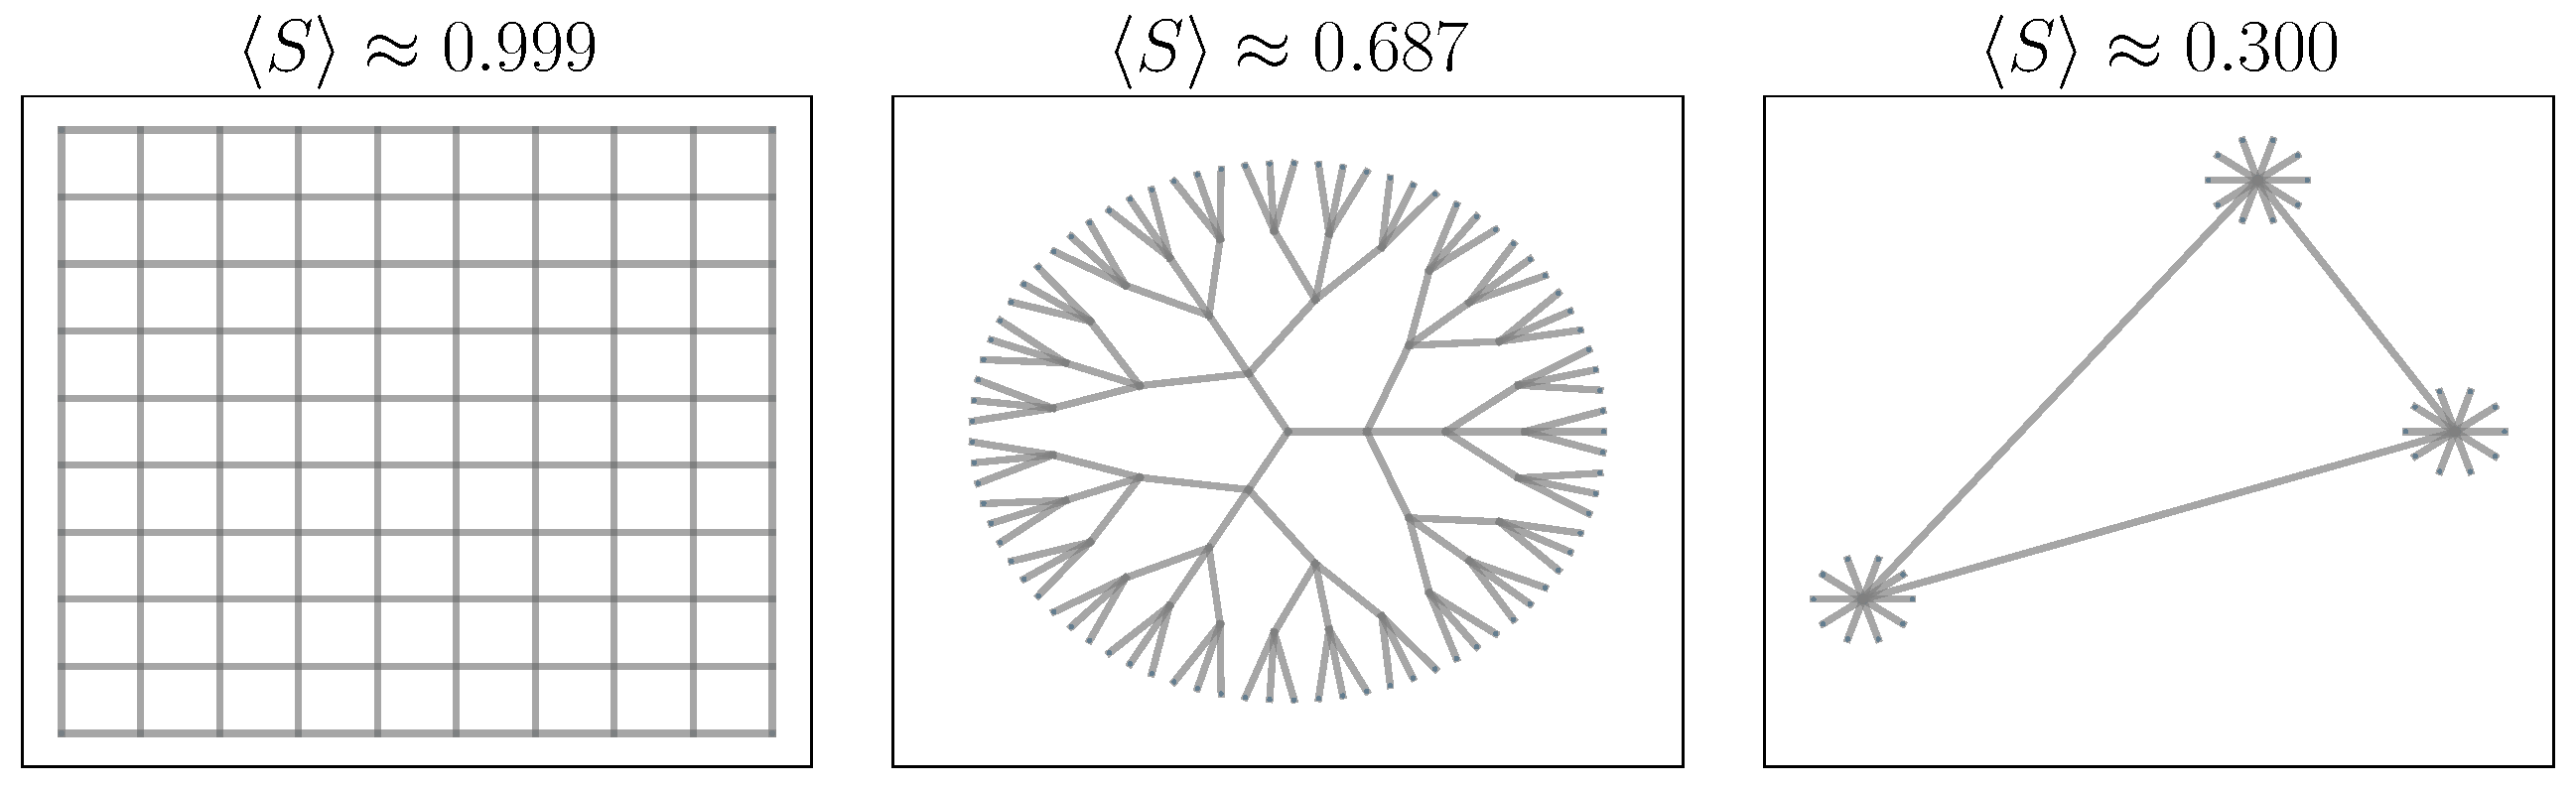
\includegraphics[width=.9\linewidth]{../figures/toy_network_examples.pdf}
			\caption{Toy models}
		\end{figure}
		
		\begin{figure}
			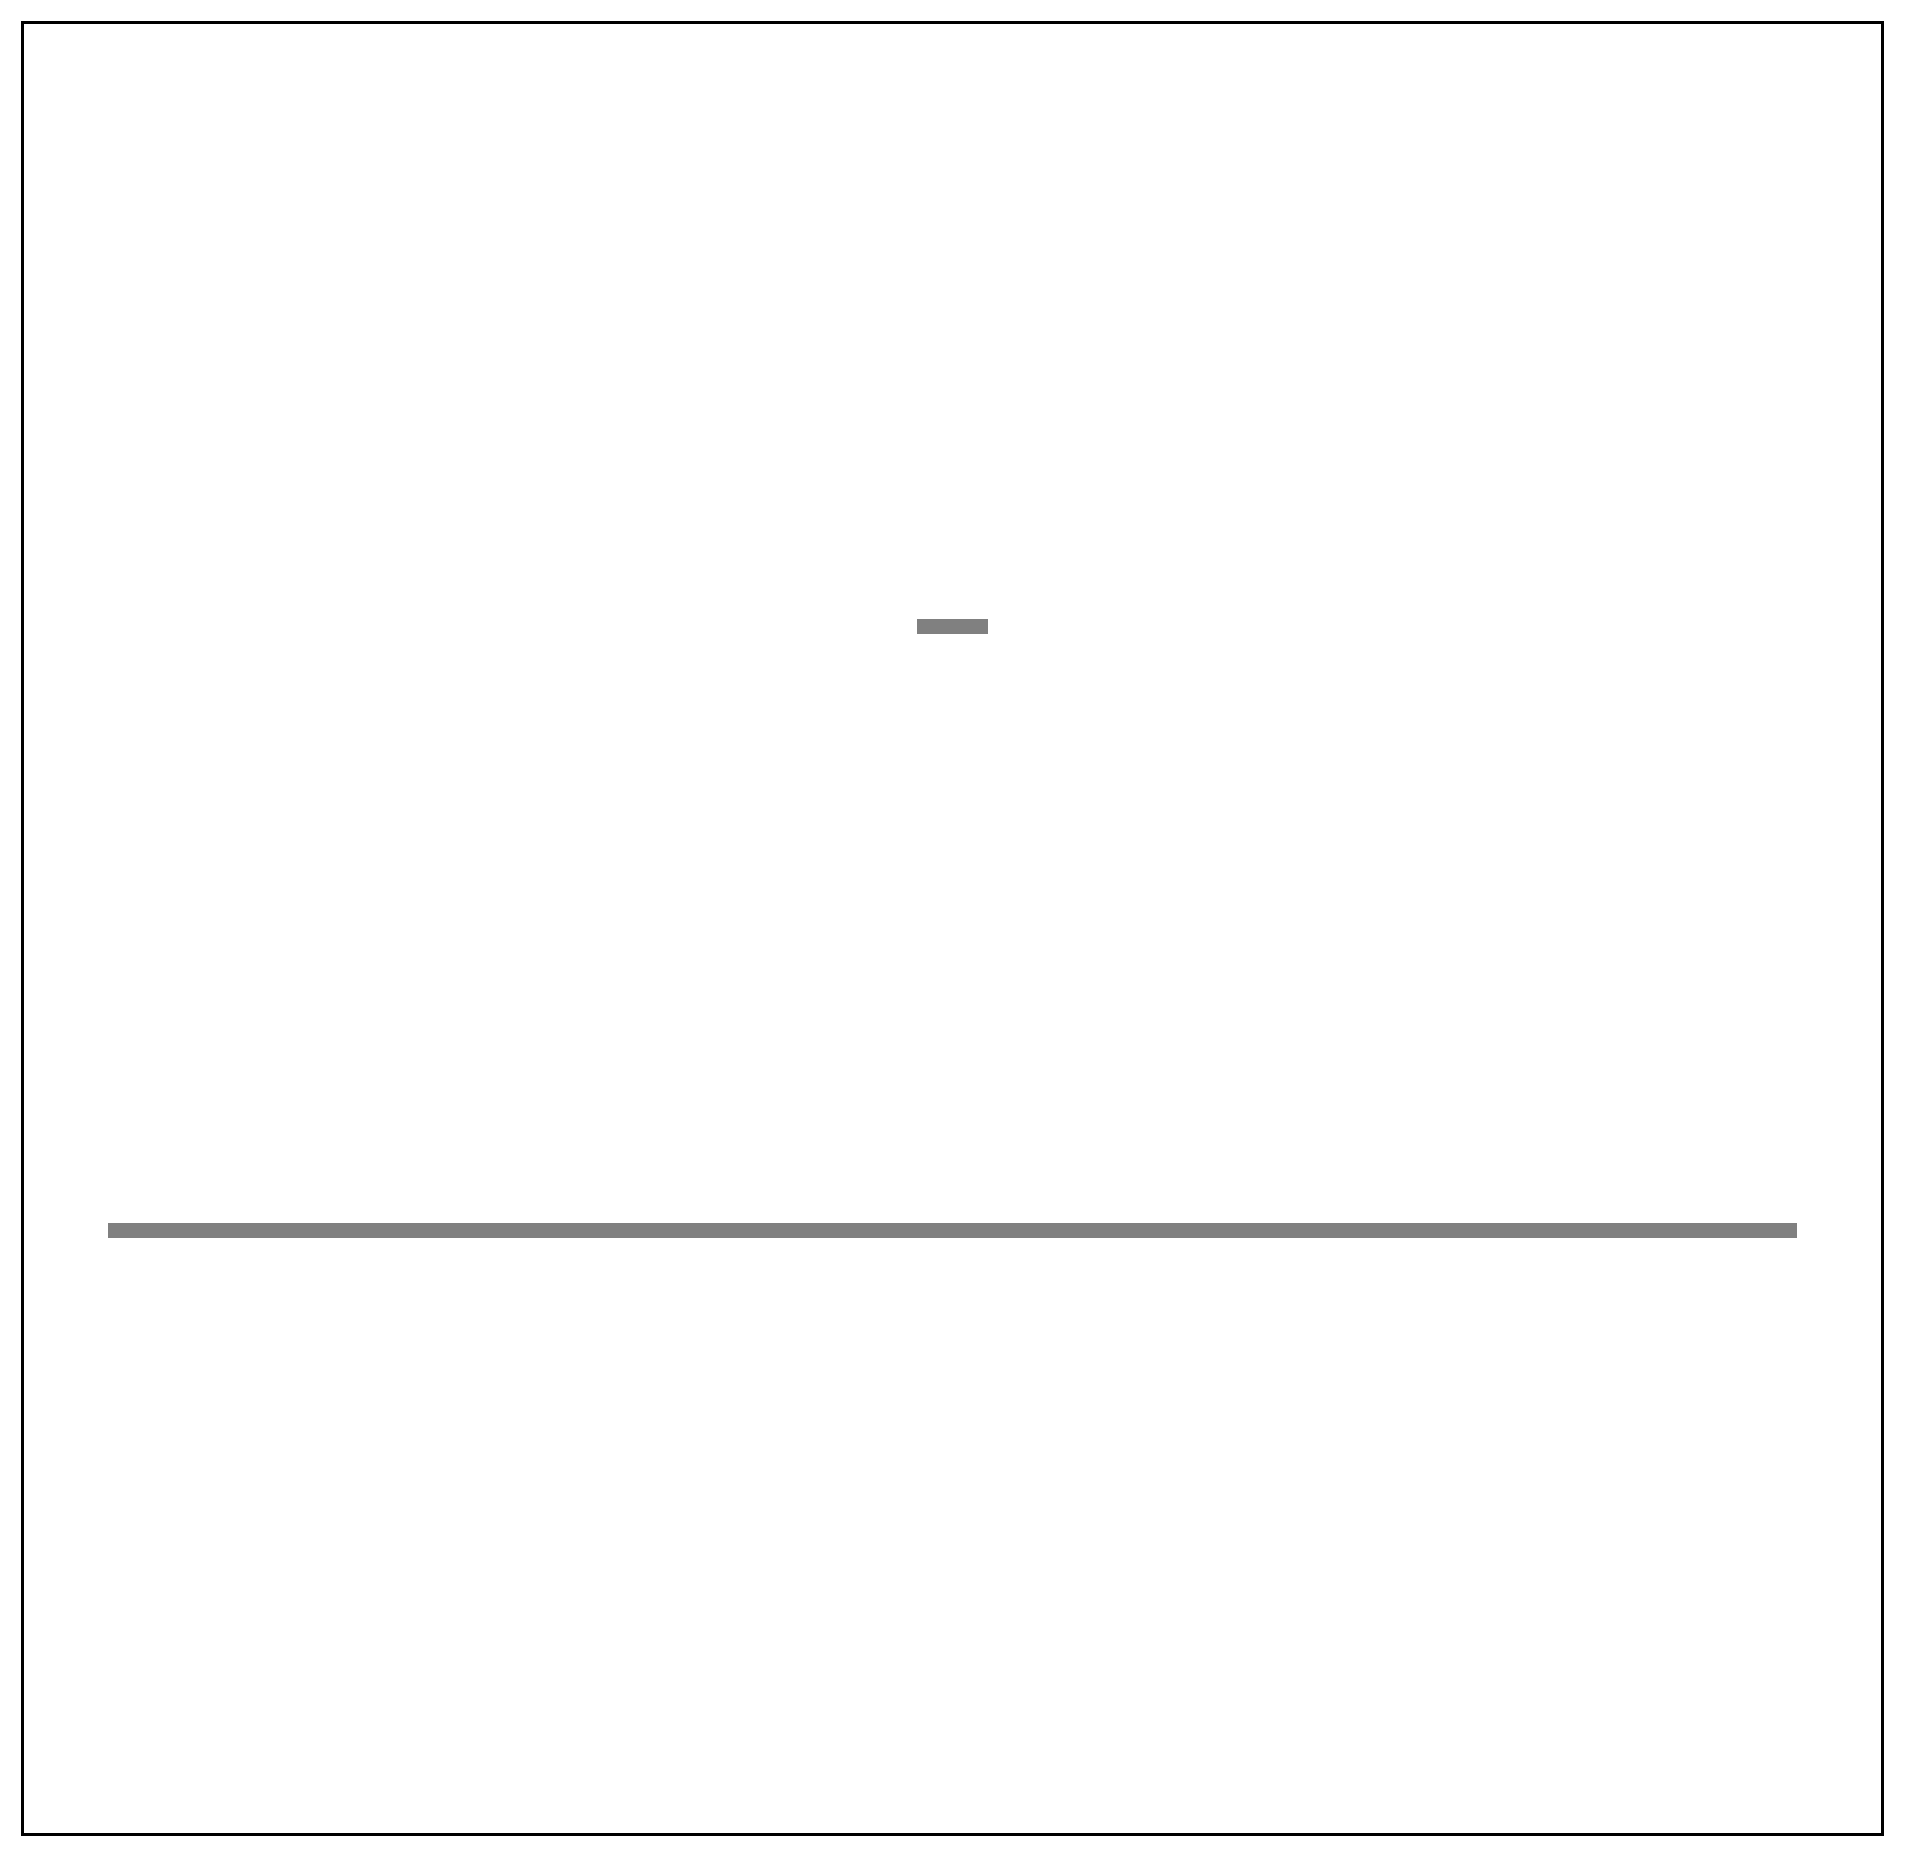
\includegraphics[width=0.25\linewidth]{../figures/breaking_example_spatial_strength.pdf}
			\caption{Showing mean spatial strength is unbounded}
		\end{figure}
	}
	
	\frame {
		\frametitle{Spatial Strength}
		\framesubtitle{Mean spatial strength on data}
		\begin{figure}
			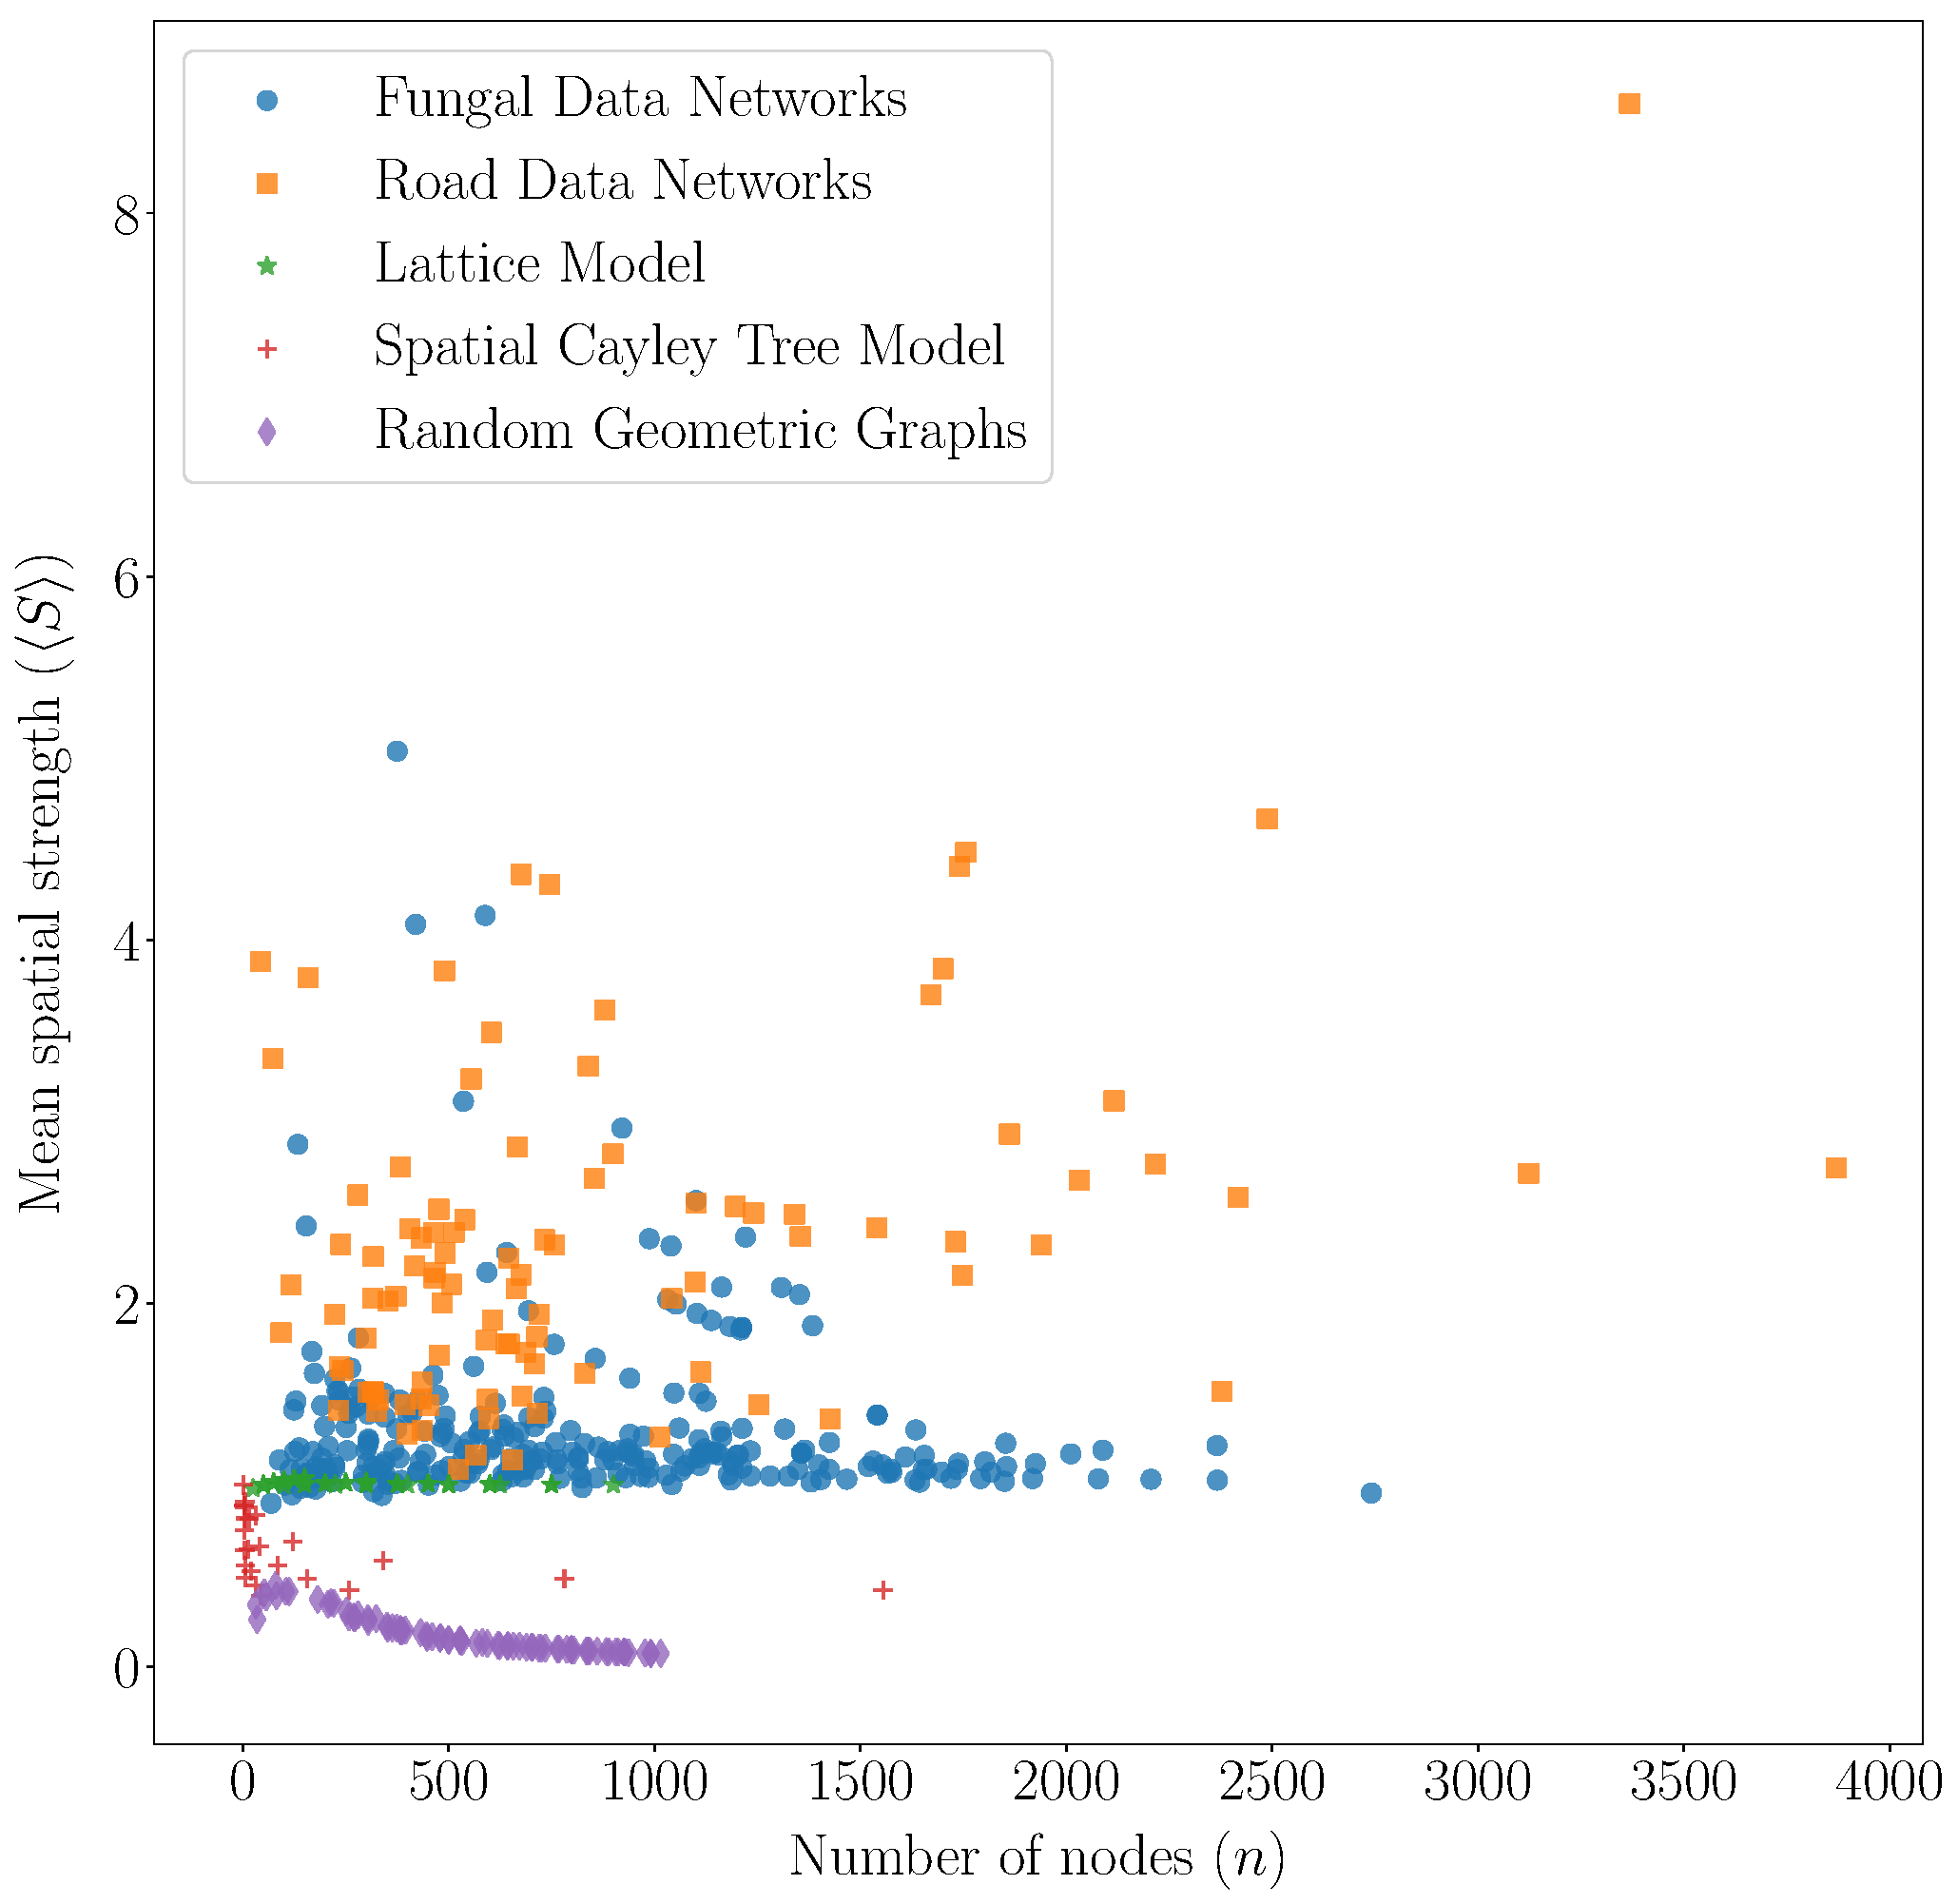
\includegraphics[width=0.65\linewidth]{../figures/spatial_scatter_1.pdf}
			\caption{Mean spatial strengths for different data organized by number of nodes}
		\end{figure}
	}
	
	\frame {
		\frametitle{Other Points}
		\begin{itemize}
			\item $\bullet$ There are other ways to think about spatial strength
			\item $\bullet$ Spatial strength assumes closer nodes should be attached and doesn't consider underlying topology
			\item $\bullet$ Try to figure out influence of deterrence function on edge formation probability
			\item $\bullet$ Further considerations for spatial configuration model
		\end{itemize}
	}
	
	\frame {
	The end!
	}
\end{document}